%%%%%%%%%%%%%%%%%%%%%%%%%%%%%%%%%%%%%%%%%%%%%%
%%%%%%%%%%%%%%%%%%%%%%%%%%%%%%%%%%%%%%%%%%%%%%
%%                                          %%
%% Important note on usage                  %%
%% -----------------------                  %%
%% This file must be compiled with PDFLaTeX %%
%% Using standard LaTeX will not work!      %%
%%                                          %%
%%%%%%%%%%%%%%%%%%%%%%%%%%%%%%%%%%%%%%%%%%%%%%
%%%%%%%%%%%%%%%%%%%%%%%%%%%%%%%%%%%%%%%%%%%%%%

%% The '3p' and 'times' class options of elsarticle are used for Elsevier CRC
\documentclass[5p]{elsarticle}
% \documentclass[3p,times]{elsarticle}
% \documentclass[3p]{elsarticle}

\usepackage[american]{babel}
\usepackage{amsmath}
\usepackage[version=3]{mhchem} 
% \usepackage{fixltx2e}
% \usepackage{refcount}
% \usepackage{siunitx}
% \usepackage{lastpage}
% \usepackage{textcomp}
\usepackage{mathtools}

\usepackage{xfrac}
\usepackage{lmodern}
\usepackage[hidelinks]{hyperref}
% \usepackage{cool}
% \usepackage{cancel}
\usepackage{microtype}
\usepackage{listings}
\usepackage{mcode}
\usepackage [autostyle, english = american]{csquotes}
\usepackage{longtable}
\usepackage{subcaption}
\usepackage{booktabs}
\usepackage{gensymb}



% \usepackage[usenames,dvipsnames,svgnames,table]{xcolor}
\usepackage{color}

\usepackage[colorinlistoftodos]{todonotes}

\usepackage[section]{placeins}


\lstset{basicstyle=\small\ttfamily,columns=fullflexible}

% \usepackage{verbatim}



% \usepackage{gensymb}
% \usepackage{enumerate}
% \usepackage{float}
% \usepackage{bm}
% \usepackage{csquotes}
% \usepackage{mathtools}
% \usepackage{natbib}
% \usepackage{biblatex}

%% The `ecrc' package must be called to make the CRC functionality available
\usepackage{ecrc}

%% The ecrc package defines commands needed for running heads and logos.
%% For running heads, you can set the journal name, the volume, the starting page and the authors

%% set the volume if you know. Otherwise `00'
\volume{00}

%% set the starting page if not 1
\firstpage{1}

%% Give the name of the journal
\journalname{Nuclear Instruments and Methods in Physics Research B}

%% Give the author list to appear in the running head
%% Example \runauth{C.V. Radhakrishnan et al.}
\runauth{A.S. Voyles et al.}

%% The choice of journal logo is determined by the \jid and \jnltitlelogo commands.
%% A user-supplied logo with the name <\jid>logo.pdf will be inserted if present.
%% e.g. if \jid{yspmi} the system will look for a file yspmilogo.pdf
%% Otherwise the content of \jnltitlelogo will be set between horizontal lines as a default logo

%% Give the abbreviation of the Journal.
\jid{nimb}
% \jid{yspmi}

%% Give a short journal name for the dummy logo (if needed)
\jnltitlelogo{Nucl Instrum Meth B}

%% Hereafter the template follows `elsarticle'.
%% For more details see the existing template files elsarticle-template-harv.tex and elsarticle-template-num.tex.

%% Elsevier CRC generally uses a numbered reference style
%% For this, the conventions of elsarticle-template-num.tex should be followed (included below)
%% If using BibTeX, use the style file elsarticle-num.bst

%% End of ecrc-specific commands
%%%%%%%%%%%%%%%%%%%%%%%%%%%%%%%%%%%%%%%%%%%%%%%%%%%%%%%%%%%%%%%%%%%%%%%%%%

%% The amssymb package provides various useful mathematical symbols
\usepackage{amssymb}
%% The amsthm package provides extended theorem environments
\usepackage{amsthm}

%% The lineno packages adds line numbers. Start line numbering with
%% \begin{linenumbers}, end it with \end{linenumbers}. Or switch it on
%% for the whole article with \linenumbers after \end{frontmatter}.
%% \usepackage{lineno}

%% natbib.sty is loaded by default. However, natbib options can be
%% provided with \biboptions{...} command. Following options are
%% valid:

%%   round  -  round parentheses are used (default)
%%   square -  square brackets are used   [option]
%%   curly  -  curly braces are used      {option}
%%   angle  -  angle brackets are used    <option>
%%   semicolon  -  multiple citations separated by semi-colon
%%   colon  - same as semicolon, an earlier confusion
%%   comma  -  separated by comma
%%   numbers-  selects numerical citations
%%   super  -  numerical citations as superscripts
%%   sort   -  sorts multiple citations according to order in ref. list
%%   sort&compress   -  like sort, but also compresses numerical citations
%%   compress - compresses without sorting
%%
%% \biboptions{comma,round}

% \biboptions{}

% if you have landscape tables
\usepackage[figuresright]{rotating}

% put your own definitions here:
%   \newcommand{\cZ}{\cal{Z}}
%   \newtheorem{def}{Definition}[section]
%   ...

% add words to TeX's hyphenation exception list
%\hyphenation{author another created financial paper re-commend-ed Post-Script}

% declarations for front matter

\usepackage{fancyvrb}
\usepackage{color}
 
\definecolor{mygreen}{rgb}{0,0.6,0}
\definecolor{mygray}{rgb}{0.5,0.5,0.5}
\definecolor{mymauve}{rgb}{0.58,0,0.82}

\lstset{ %
  backgroundcolor=\color{white},   % choose the background color
  basicstyle=\footnotesize,        % size of fonts used for the code
  breaklines=true,                 % automatic line breaking only at whitespace
  captionpos=b,                    % sets the caption-position to bottom
  commentstyle=\color{mygreen},    % comment style
  escapeinside={\%*}{*)},          % if you want to add LaTeX within your code
  keywordstyle=\color{blue},       % keyword style
  stringstyle=\color{mymauve},     % string literal style
}

% Sin and Cos with auto-parentheses 
\newcommand{\sinp}[1]{\sin{\left( #1\right)}}
\newcommand{\cosp}[1]{\cos{\left( #1\right)}}
\newcommand{\expp}[1]{\exp{\left( #1\right)}}
\newcommand{\sinhp}[1]{\sinh{\left( #1\right)}}
\newcommand{\lnp}[1]{\ln{\left( #1\right)}}
\newcommand{\pp}[1]{\left( #1\right)}
\newcommand{\sci}[2]{ #1 \cdot 10^{#2}\ }
\newcommand{\angstrom}{\mbox{\normalfont\AA}}
\newcommand{\norm}[1]{\lVert #1 \rVert}


\newcommand{\colornote}[1]{\textcolor{red}{ COMMENT\large\footnote{\textcolor{red}{#1}}}}

\newcommand{\comment}[1]{\todo[color=blue!20!white,inline]{ASV: #1}} 




\makeatletter
% Make common definition of mean
\newcommand*\mean[1]{\overline{#1\raisebox{3mm}{}}}

\makeatother




\begin{document}

\begin{frontmatter}

%% Title, authors and addresses

%% use the tnoteref command within \title for footnotes;
%% use the tnotetext command for the associated footnote;
%% use the fnref command within \author or \address for footnotes;
%% use the fntext command for the associated footnote;
%% use the corref command within \author for corresponding author footnotes;
%% use the cortext command for the associated footnote;
%% use the ead command for the email address,
%% and the form \ead[url] for the home page:
%%
\title{Determination of the \ce{^{64}Zn},\ce{^{47}Ti}(n,p) Cross-Sections using a DD Neutron Generator for Medical Isotope Studies}

% \title{(n,p) Cross-Section Measurements for \ce{^{64}Cu} and \ce{^{47}Sc} via DD Neutron Generator\tnoteref{label1}}
%% \tnotetext[label1]{}
%% \author{Name\corref{cor1}\fnref{label2}}
%% \ead{email address}
%% \ead[url]{home page}
%% \fntext[label2]{}
%% \cortext[cor1]{}
%% \address{Address\fnref{label3}}
%% \fntext[label3]{}

% \dochead{Short}
%% Use \dochead if there is an article header, e.g. \dochead{Short communication}

% \title{NE290A - Homework \#04}
% \date{29 April, 2016}

% \author[rvt]{C.V. ̃Radhakrishnan\corref{cor1}\fnref{fn1}}
\author[ucb]{A.S. Voyles \corref{cor1}}
\ead{andrew.voyles@gmail.com}

\author[lbl]{M.S. Basunia}

\author[lbl]{J.C. Batchelder}

\author[llnl]{J.D. Bauer}

\author[ucb,lbl]{L.A. Bernstein}

\author[ucb]{E.F. Matthews}

\author[geo,eps]{D. Rutte}

\author[ucb]{M.A. Unzueta}

\author[ucb]{K.A. van Bibber}



% \author[lbl]{K. ̃Bazargan\fnref{fn2}}
% \ead{kaveh@river-valley.com}



%% use optional labels to link authors explicitly to addresses:
%% \author[label1,label2]{<author name>}
%% \address[label1]{<address>}
%% \address[label2]{<address>}

\cortext[cor1]{Corresponding author}
% \cortext[cor2]{Principal corresponding author}
% \fntext[fn1]{This is the specimen author footnote.}
% \fntext[fn2]{Another author footnote, but a little more longer.}

% \address[ucb]{Department of Nuclear Engineering, University of California, Berkeley, Etcheverry Hall, 2521 Hearst Ave, Berkeley, CA 94709}
% \address[lbl]{Lawrence Berkeley National Laboratory,  1 Cyclotron Rd, Berkeley, CA 94720}
% \address[llnl]{Lawrence Livermore National Laboratory, 7000 East Ave, Livermore, CA 94550}

\address[ucb]{Department of Nuclear Engineering, University of California, Berkeley, Berkeley CA, 94720 USA}
\address[lbl]{Lawrence Berkeley National Laboratory,  Berkeley CA, 94720 USA}
\address[llnl]{Lawrence Livermore National Laboratory, Livermore CA, 94551 USA}
\address[geo]{Berkeley Geochronology Center, Berkeley CA,  94709  USA}
\address[eps]{Department of Earth and Planetary Sciences, University of California, Berkeley, Berkeley CA,  94720  USA}



% \author{Andrew Voyles}

% \address{Nuclear Engineering, University of California Berkeley, Berkeley, CA 94709, USA.}



\begin{abstract}

%\comment{Use DD or DD as convention?}



% \comment{Need Daniel's middle initial} - he doesn't have one







Cross sections for the \ce{^{47}Ti}(n,p)\ce{^{47}Sc} and \ce{^{64}Zn}(n,p)\ce{^{64}Cu} reactions have been measured for quasi-monoenergetic DD neutrons produced by the UC Berkeley High Flux Neutron Generator. The study was motivated by interest in the production of \ce{^{47}Sc} and \ce{^{64}Cu} as emerging medical isotopes. The cross sections were measured in ratio to the \ce{^{113}In}(n,n')\ce{^{113m}In} and \ce{^{115}In}(n,n')\ce{^{115m}In} inelastic scattering reactions on co-irradiated indium samples. Post-irradiation counting using an HPGe and LEPS detectors allowed for cross section determination to within 6\% uncertainty. The cross section were determined with lower uncertainty than existing measurements and are found to be  in good agreement with the literature and theoretical values. This work highlights the utility of using D-D plasma-based neutron sources, for a host of nuclear data measurements and potentially for the production of radionuclides for medical applications.


\comment{The abstract is now nicely short and sweet, but should it be expanded at all?}

\comment{For my corresponding author email, should I list my Gmail (more permanent) or my Berkeley / LBL address (more professional)?}


\end{abstract}

% \begin{keyword}
%% keywords here, in the form: keyword \sep keyword

%% MSC codes here, in the form: \MSC code \sep code
%% or \MSC[2008] code \sep code (2000 is the default)

% \end{keyword}

\end{frontmatter}

%%
%% Start line numbering here if you want
%%
% \linenumbers

\listoftodos


%% main text 
\section{Introduction} \label{sec:intro}

%
% If we want to mention in-situ-production
%
%
% e.g.:In-situ production (I always figured this is what is so great, correct me if I am wrong) of radioactive nuclides is an emerging method for radiation therapy in nuclear medicine (e.g., cite some recent review paper). It is based on doping the malignant target tissue with a stable nuclide which is then activated in-situ by neutron irradiation. Following decay is focused on the target tissue. Advantages compared to conventional radiation therapy are the reduction of damage to surrounding cells, … short range, … . Currently development of this technique is hampered by the lack of fundamental cross section data for various isotopes.

\comment{Add an initial \enquote{punchline} to  clarify the motivation?}

\comment{Per Mauricio, does 2.7 MeV count as high energy? While fast, I would consider this to still be definitely in the low-energy regime, compared to spallation, etc.}


A series of experiments are being conducted at UC Berkeley to measure low-energy neutron-induced production cross sections for a range of emerging medical radioisotopes, as many of these cross sections currently have not been measured, or possess significant uncertainties.   One potential method for producing many of these isotopes is the use of (n,p) reactions via neutron beams from DD neutron generators. Direct neutron activation, using a DD neutron generator, allows for more precise cross section measurements than time-of-flight methods, and potentially offers a proliferation-resistant pathway for radioisotope production. Neutron activation can provide several advantages over charged-particle reactions from a targetry perspective. Notably, the higher penetration of neutrons allows for the use of thick target designs, which can improve production throughput and greatly simplifies target cooling considerations. More importantly, low-energy neutron reactions can be used to prevent competing reaction channels in a charged-particle reaction which would otherwise contaminate the product specific activity.

The present work focuses on the (n,p) production cross section measurements of \ce{^{64}Cu} and \ce{^{47}Sc}. Copper-64  ($t_{1/2}$ = 12.7 h) undergoes $\beta^+$ decay (61.5\% branching ratio) to \ce{^{64}Ni} or $\beta^-$ decay (38.5\% branching ratio) to \ce{^{64}Zn}. The emitted 190-keV $\beta^-$ particle makes this an  attractive short-ranged therapeutic radionuclide, which also has the possibility for simultaneous positron emission tomography (PET) imaging  due to the positron emission branch (for real-time dose monitoring and verification),  making \ce{^{64}Cu} particularly attractive for emerging radiation therapy protocols. In addition, copper radiochemistry is well developed, and many existing ligands and carriers may be used for selective delivery of the radionuclide to different sites in patients.

Scandium-47 ($t_{1/2}$ = 3.35 d) undergoes $\beta^-$ decay to \ce{^{47}Ti}, emitting a high-intensity 159-keV gamma ray in the process. This radionuclide is  attractive as an emerging diagnostic isotope, due to the similarity of the emitted gamma ray to that of the more well-established \ce{^{99m}Tc}. However, due to the short half-life  and dwindling supplies of \ce{^{99m}Tc}, \ce{^{47}Sc} stands poised as a potential solution to this shortage, due to its longer half-life and multiple production pathways without the need for highly enriched uranium.

\comment{Adding a short paragraph from Mauricio explaining benefits of DD generators vs other neutron sources?}

\comment{Per Daniel, add a short summary of results here?}

Current methodology in radiochemistry has been proven to successfully recover upwards of 95\% of produced \ce{^{64}Cu} and \ce{^{47}Ti} from solid target designs, without the need for additional carrier. By expanding the base of efficient reaction pathways, great advances can be made in making production of medical radionuclides more efficient and affordable for those in need.

\comment{Should this last paragraph be moved to the results and discussion at the end of the paper?}





\section{Experiment}\label{sec:experiment}



\subsection{Neutron source}\label{sec:n_source}

\comment{Regex to replace all hard figure references with LaTeX cross-references}

Neutron activation was carried out via irradiation in the High-Flux Neutron Generator (HFNG), a DD neutron generator at the University of California, Berkeley, seen in  \autoref{fig:hfng_a}. This generator extracts deuterium ions from an RF-heated deuterium plasma through a nozzle, whose shape was designed to form a flat-profile beam 5 mm in diameter. This deuterium beam is incident upon a water-cooled, self-loading titanium-coated copper target, where the titanium layer acts as a reaction surface for DD fusion, producing neutrons with a well-known energy distribution as a function of lab emission angle \cite{Liskien_Paulsen_1973}. Within the center of the target (at 8 mm from the DD reaction surface), samples may be inserted prior to  HFNG startup. \autoref{fig:hfng_b} displays the target setup. At the time of the presented experiments, the machine operated under nominal conditions of a 100 kV deuterium beam extracted at 1.5 mA, creating a fluence of approximately  $\sci{1.3}{7}$ neutrons/cm$^2$ on the target.


\comment{Karl: Comment or question primarily to Lee: Is it conventional to put photographs of equipment in PRC? I'm not sure it is; yes certainly for NIM, but not sure about PRC.}


\comment{Note: all images here were included at nearly full-size. They obviously need to be reduced in size, but I included them here larger the needed, so they wouldn't be pixelated if enlarged. Shrink away :)}


\begin{figure}
 \centering
%  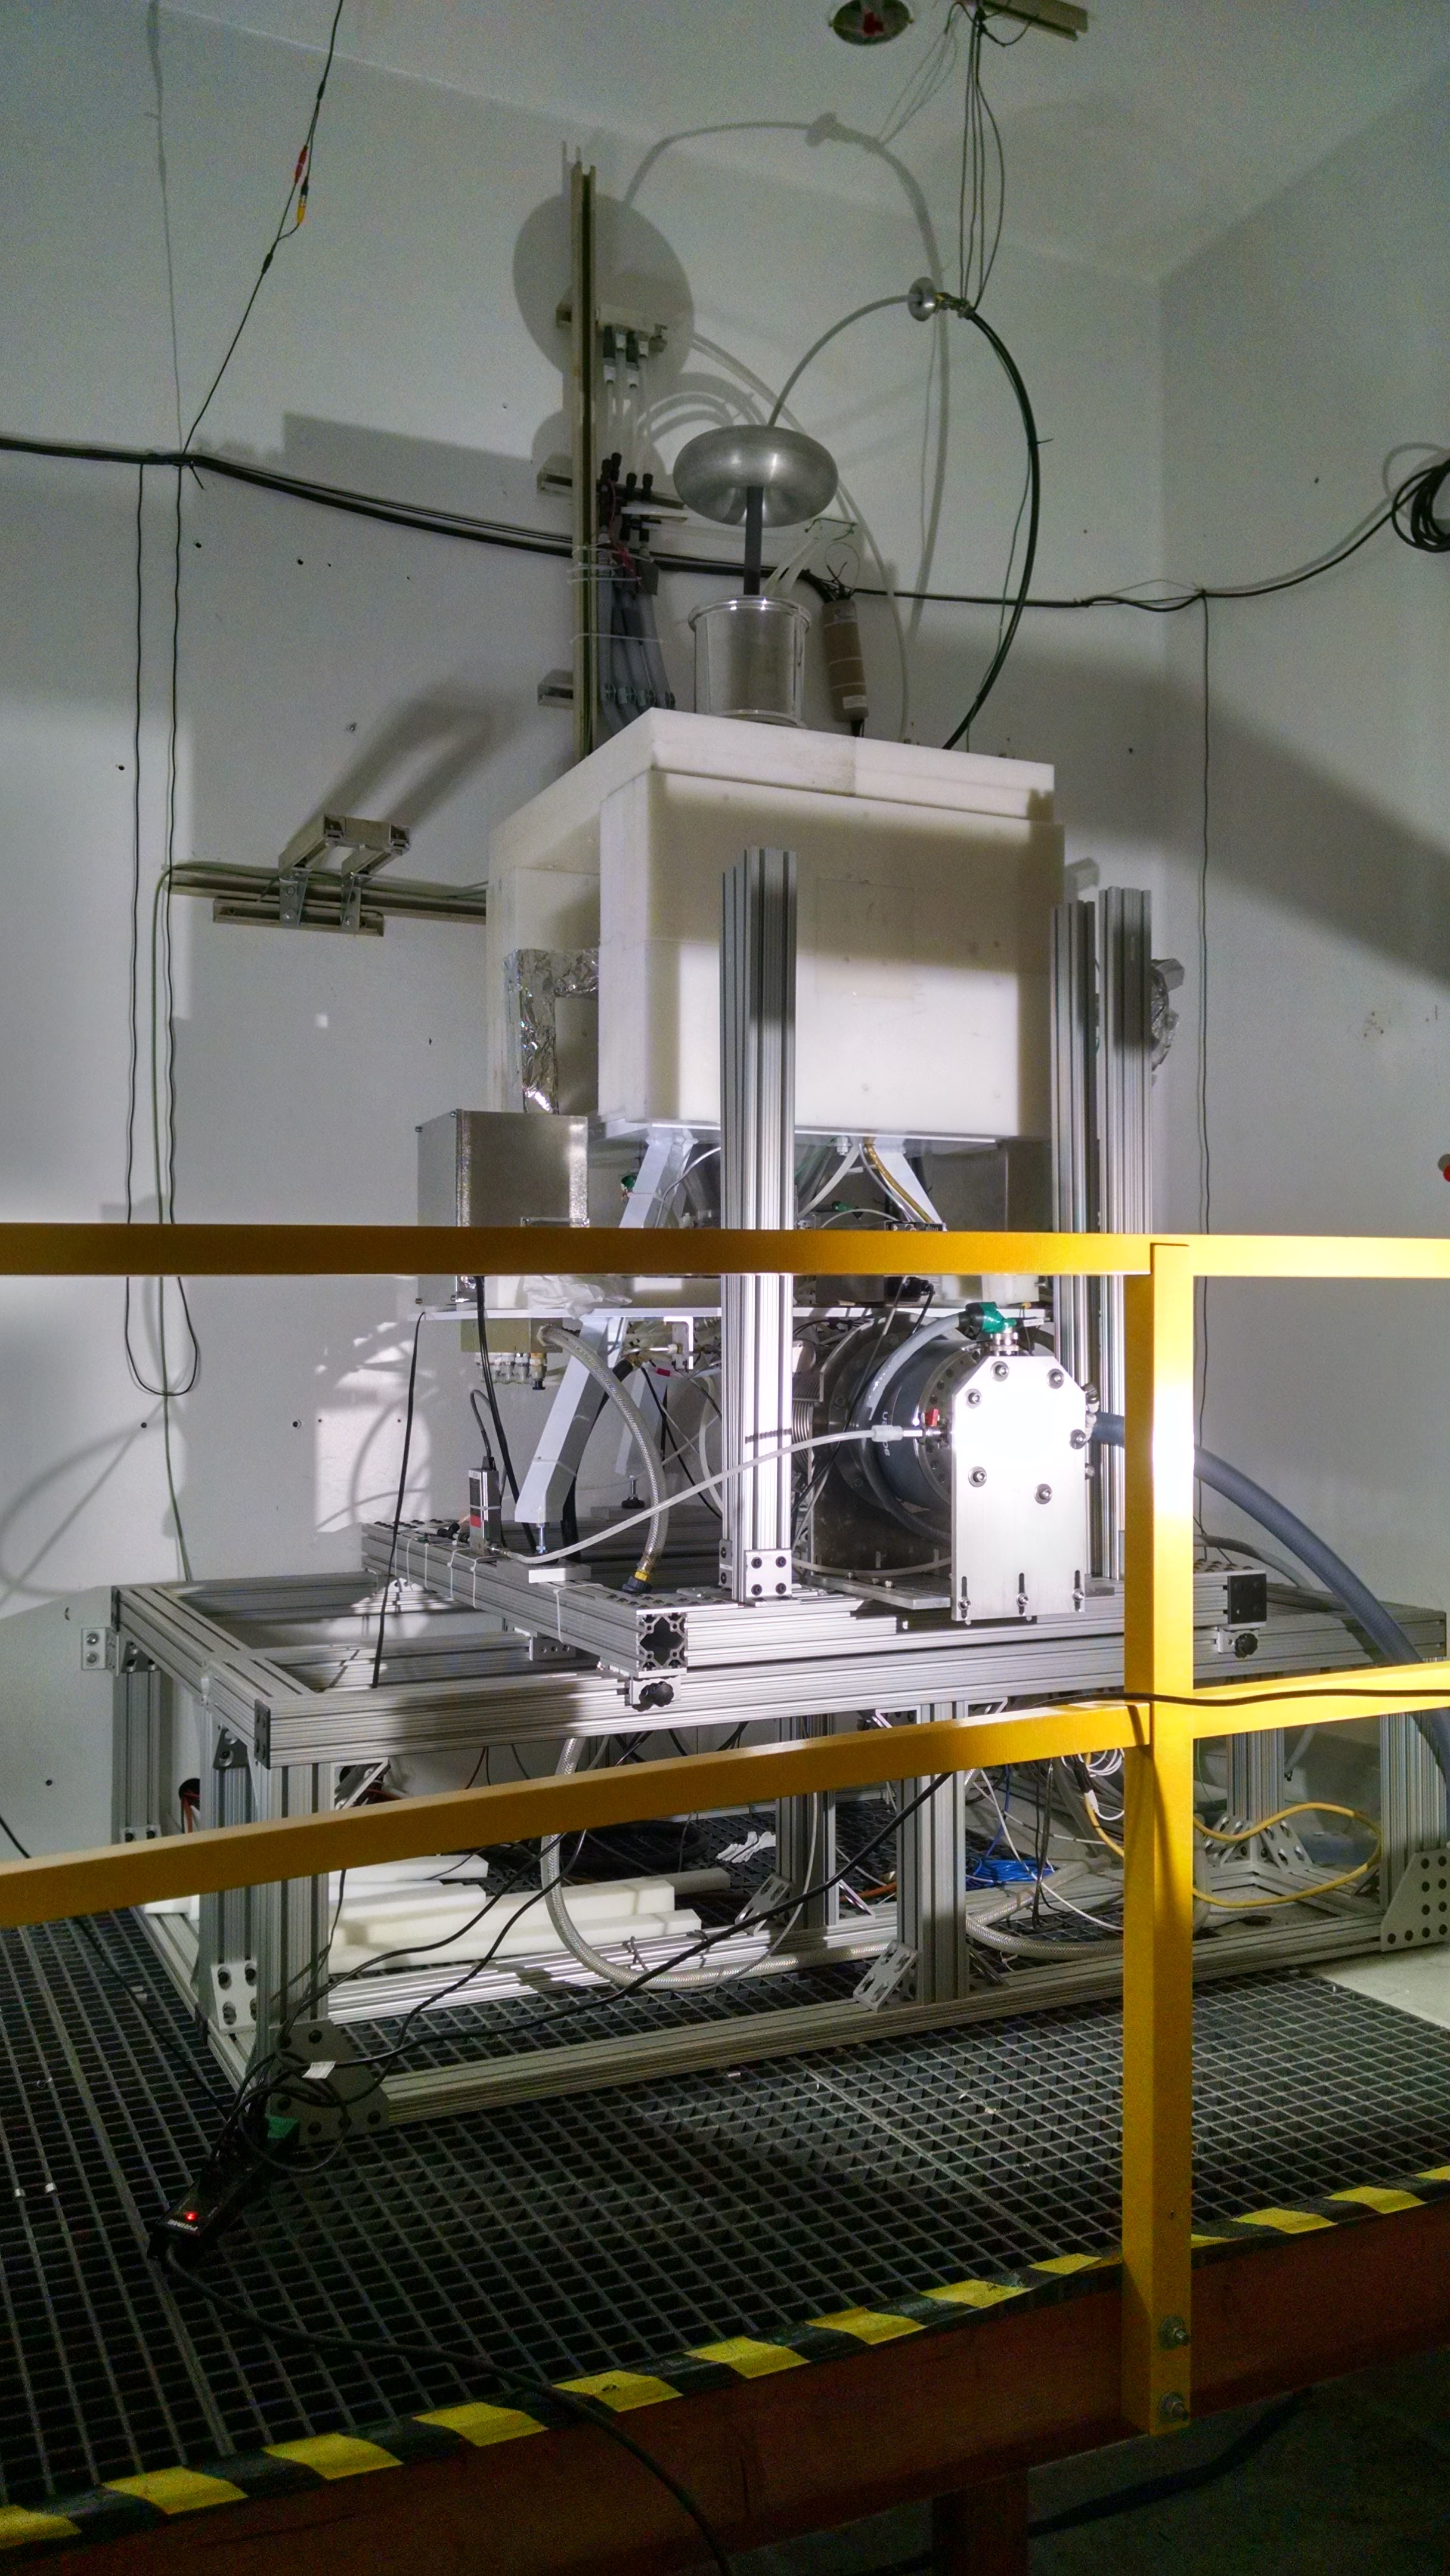
\includegraphics[width=\columnwidth]{./figures/IMG_20160531_183154957_HDR.jpg}
 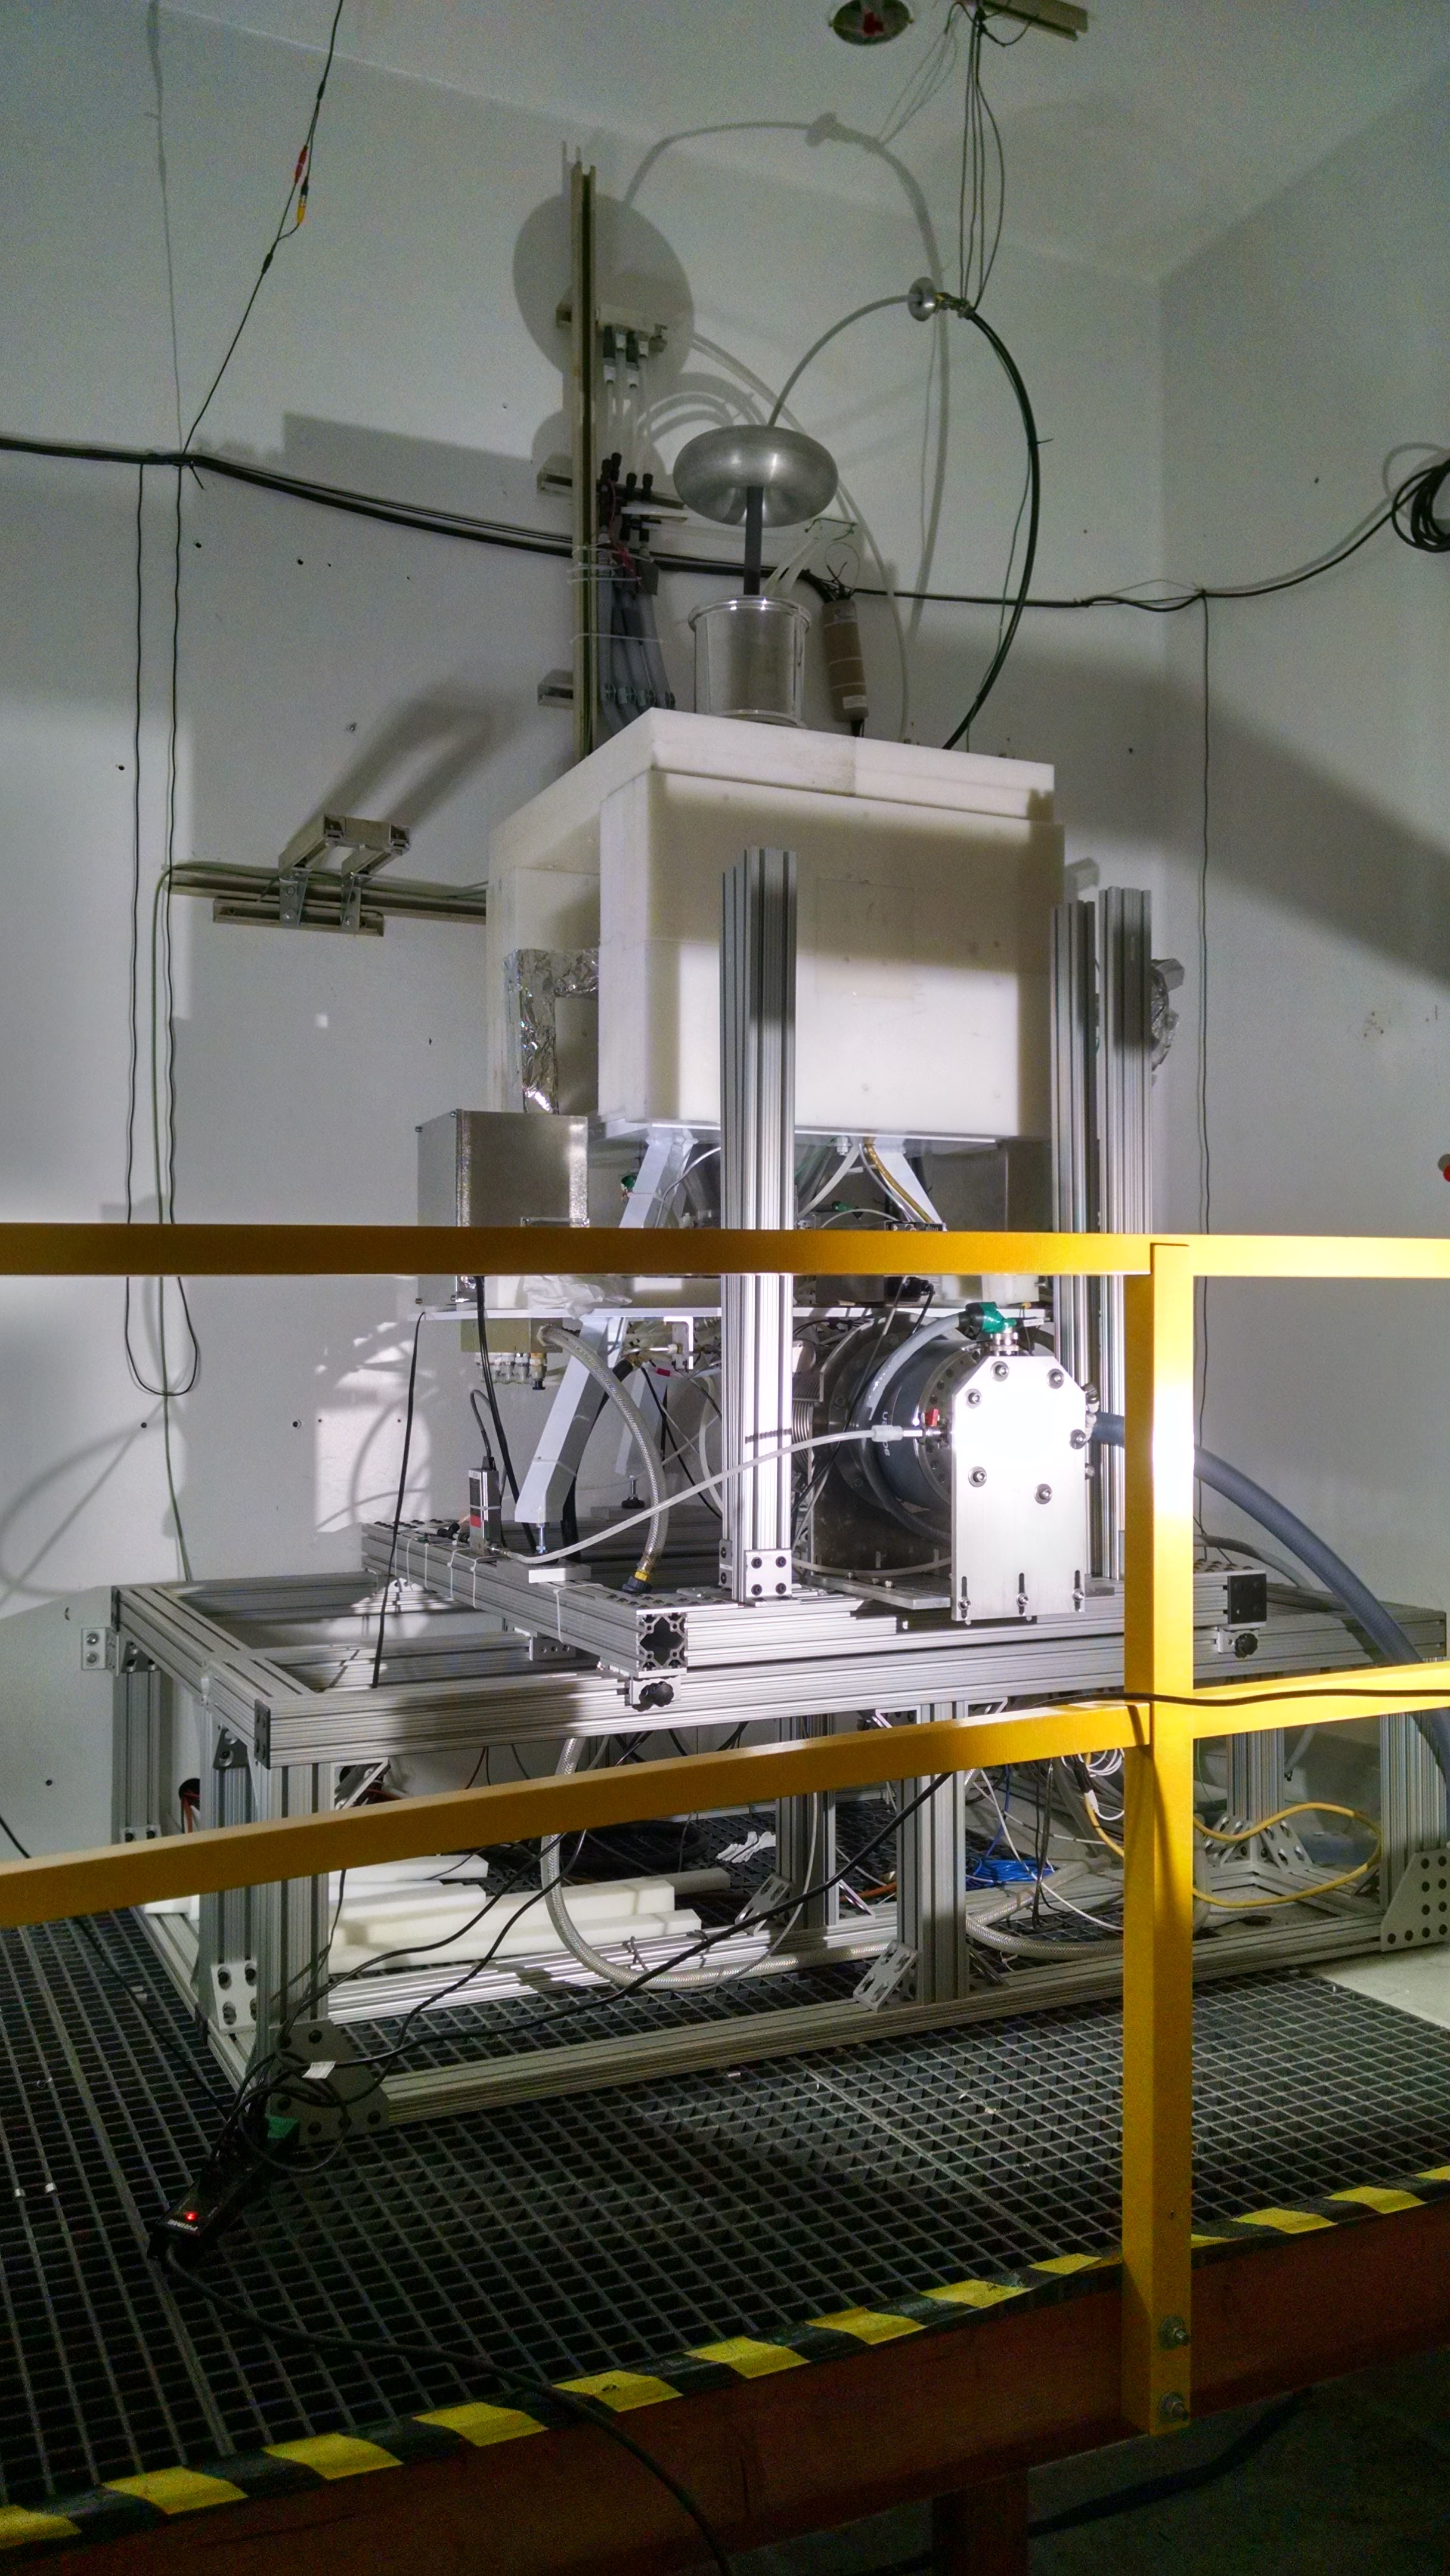
\includegraphics[scale=0.06]{./figures/IMG_20160531_183154957_HDR.jpg}
 % IMG_20160531_183154957_HDR.jpg: 2432x4320 pixel, 72dpi, 85.80x152.40 cm, bb=0 0 2432 4320
 \caption{Alternate HFNG picture - \color{red}{use this or  \autoref{fig:hfng_a}?}}
 \label{fig:alt_HFNG}
\end{figure}

\begin{figure*}
    \centering
    \begin{subfigure}[t]{0.4\textwidth}
        \centering
%         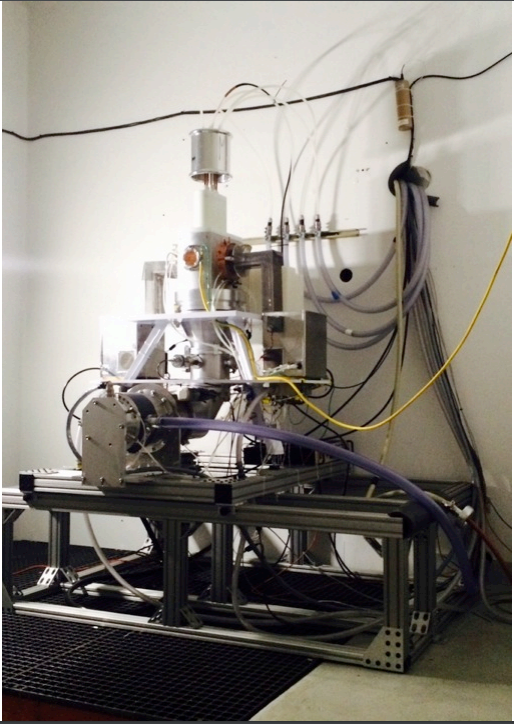
\includegraphics[width=\columnwidth]{./figures/Capture.PNG}
        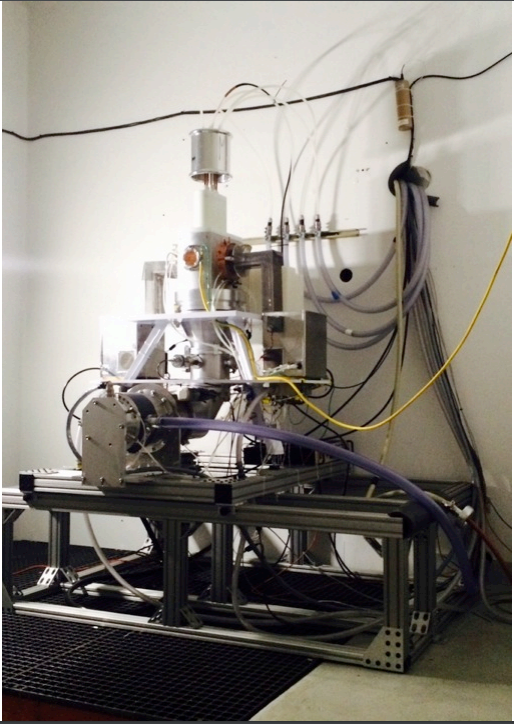
\includegraphics[height=3in]{./figures/Capture.PNG}
        \caption{The UC Berkeley High-Flux Neutron Generator,}
        \label{fig:hfng_a}
    \end{subfigure}%
    ~ 
    \begin{subfigure}[t]{0.4\textwidth}
        \centering
%         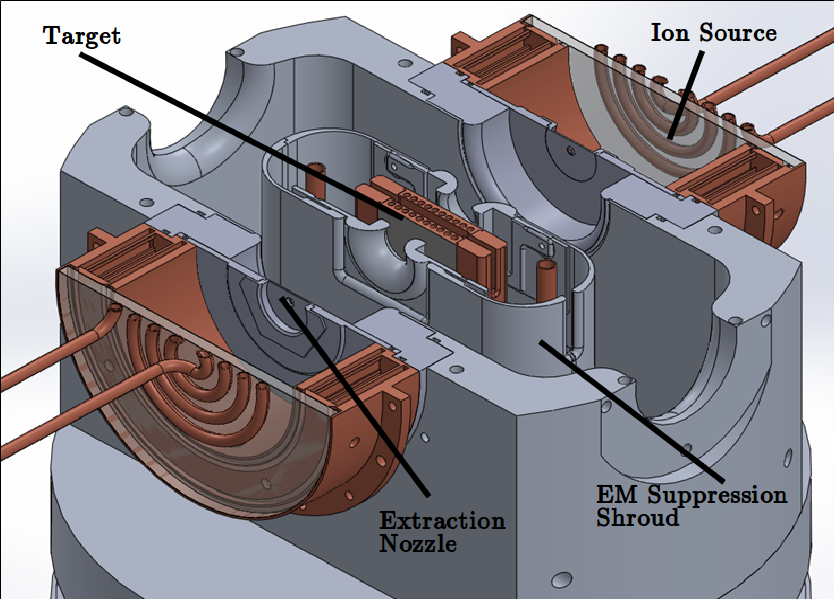
\includegraphics[width=\textwidth]{./figures/target2.png}
        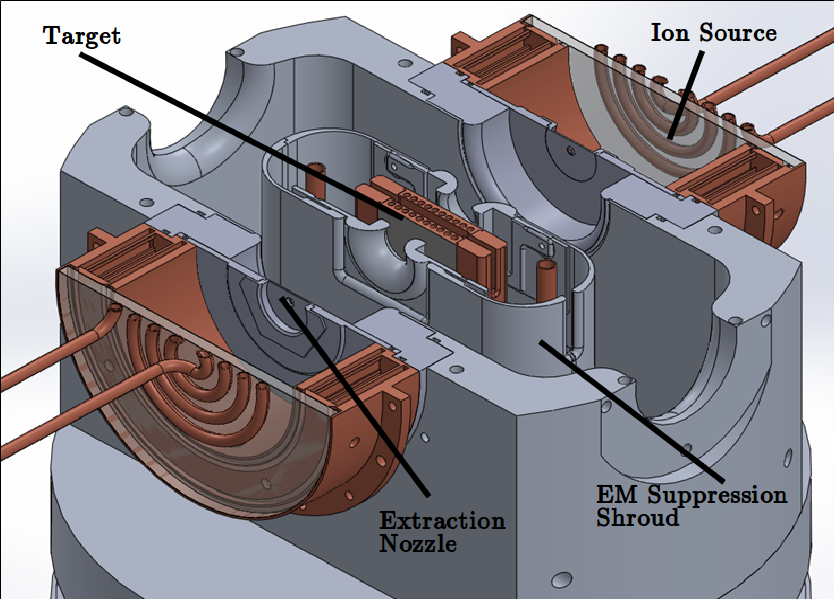
\includegraphics[height=2in]{./figures/target2.png}
        \caption{Cutaway of the target chamber.}
                \label{fig:hfng_b}
    \end{subfigure}
    \caption{Note: the ion source is approximately 20 cm in diameter.}
     \label{fig:main_HFNG}
\end{figure*}


\subsection{Sample loading}\label{sec:sample_loading}

Direct activation of a thin foil can be used for high-fidelity measurement of neutron-induced reactions, through subsequent decay spectroscopy. This method can provide cross sections with far lower uncertainty than neutron time-of-flight measurements, but is heavily reliant upon precisely quantifying the neutron fluence incident upon a loaded target. To avoid the introduction of this large uncertainty, 0.5-mm thin Indium foils were co-loaded along with each target foil for irradiation, with all production cross sections thus measured relative to the well-characterized \ce{^{113}In}(n,n')\ce{^{113m}In} and \ce{^{115}In}(n,n')\ce{^{115m}In} dosimetry standard reactions. In addition, over the energy region spanned by the DD emission spectrum, the \ce{^{113}In}(n,n')\ce{^{113m}In} and \ce{^{115}In}(n,n')\ce{^{115m}In} reaction cross sections are nearly constant, which greatly simplifies the (Zn/In) and (Ti/In) ratio measurements. The use of this well-established ratio method removes the fluence dependence from all cross-section calculations, removing the largest source of systematic uncertainty in activation.


\begin{figure*}
    \centering
    \begin{subfigure}[t]{0.3\textwidth}
        \centering
%         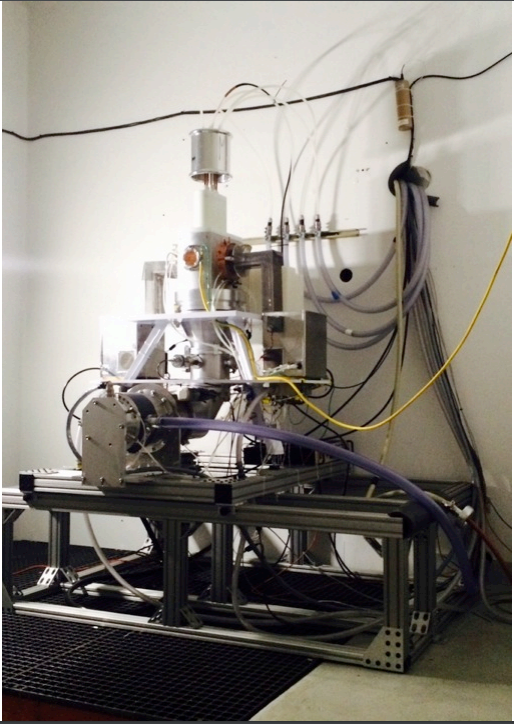
\includegraphics[width=\columnwidth]{./figures/Capture.PNG}
        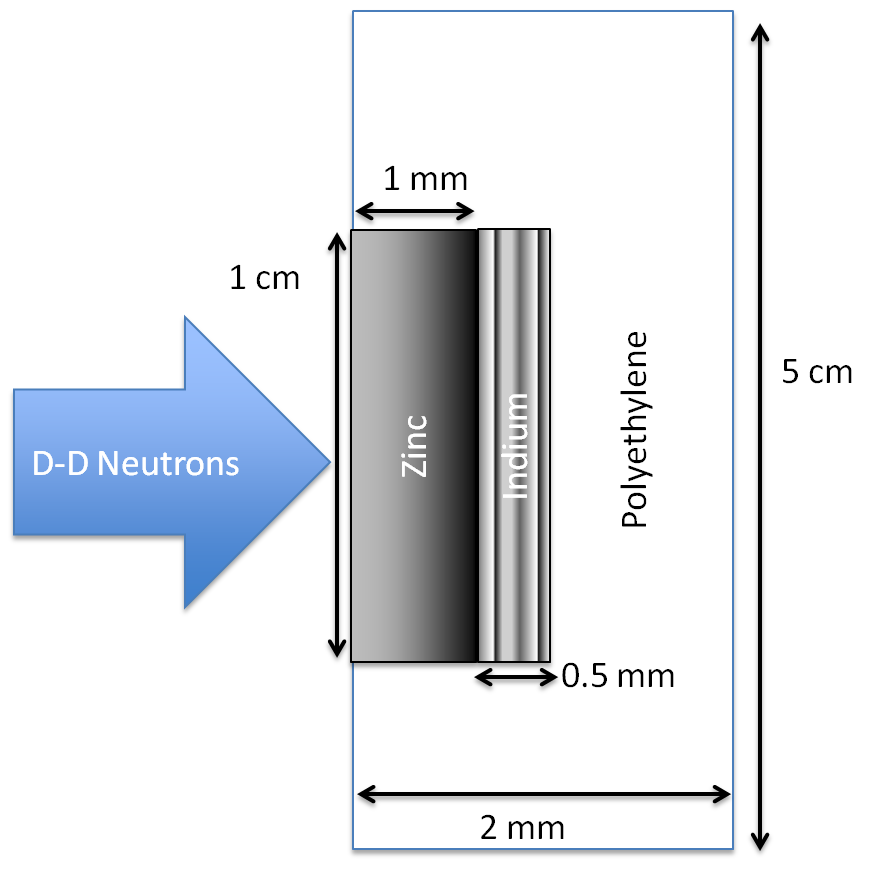
\includegraphics[height=2in]{./figures/foils.png}
        \caption{Schematic (not drawn to scale) of the foil co-loading holder for the Berkeley HFNG,}
        \label{fig:holder_a}
    \end{subfigure}%
    ~ 
    \begin{subfigure}[t]{0.3\textwidth}
        \centering
%         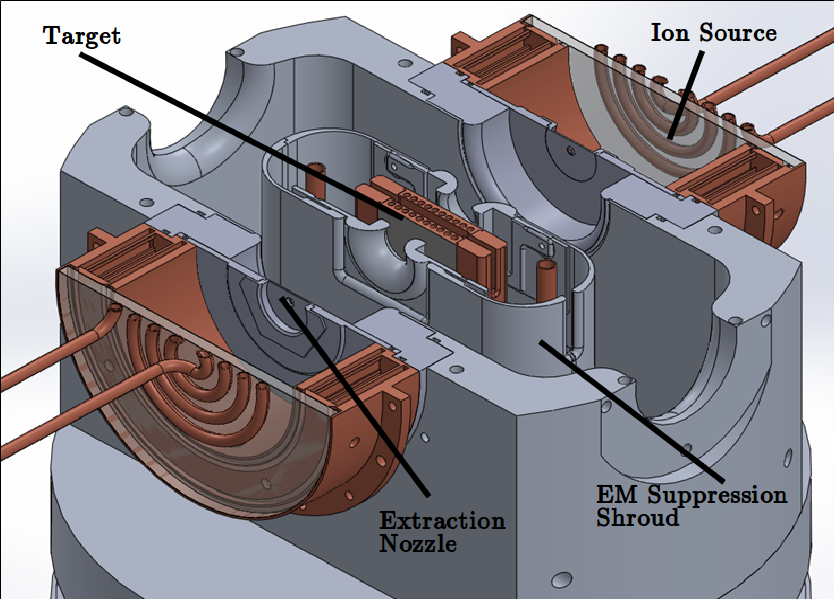
\includegraphics[width=\textwidth]{./figures/target2.png}
        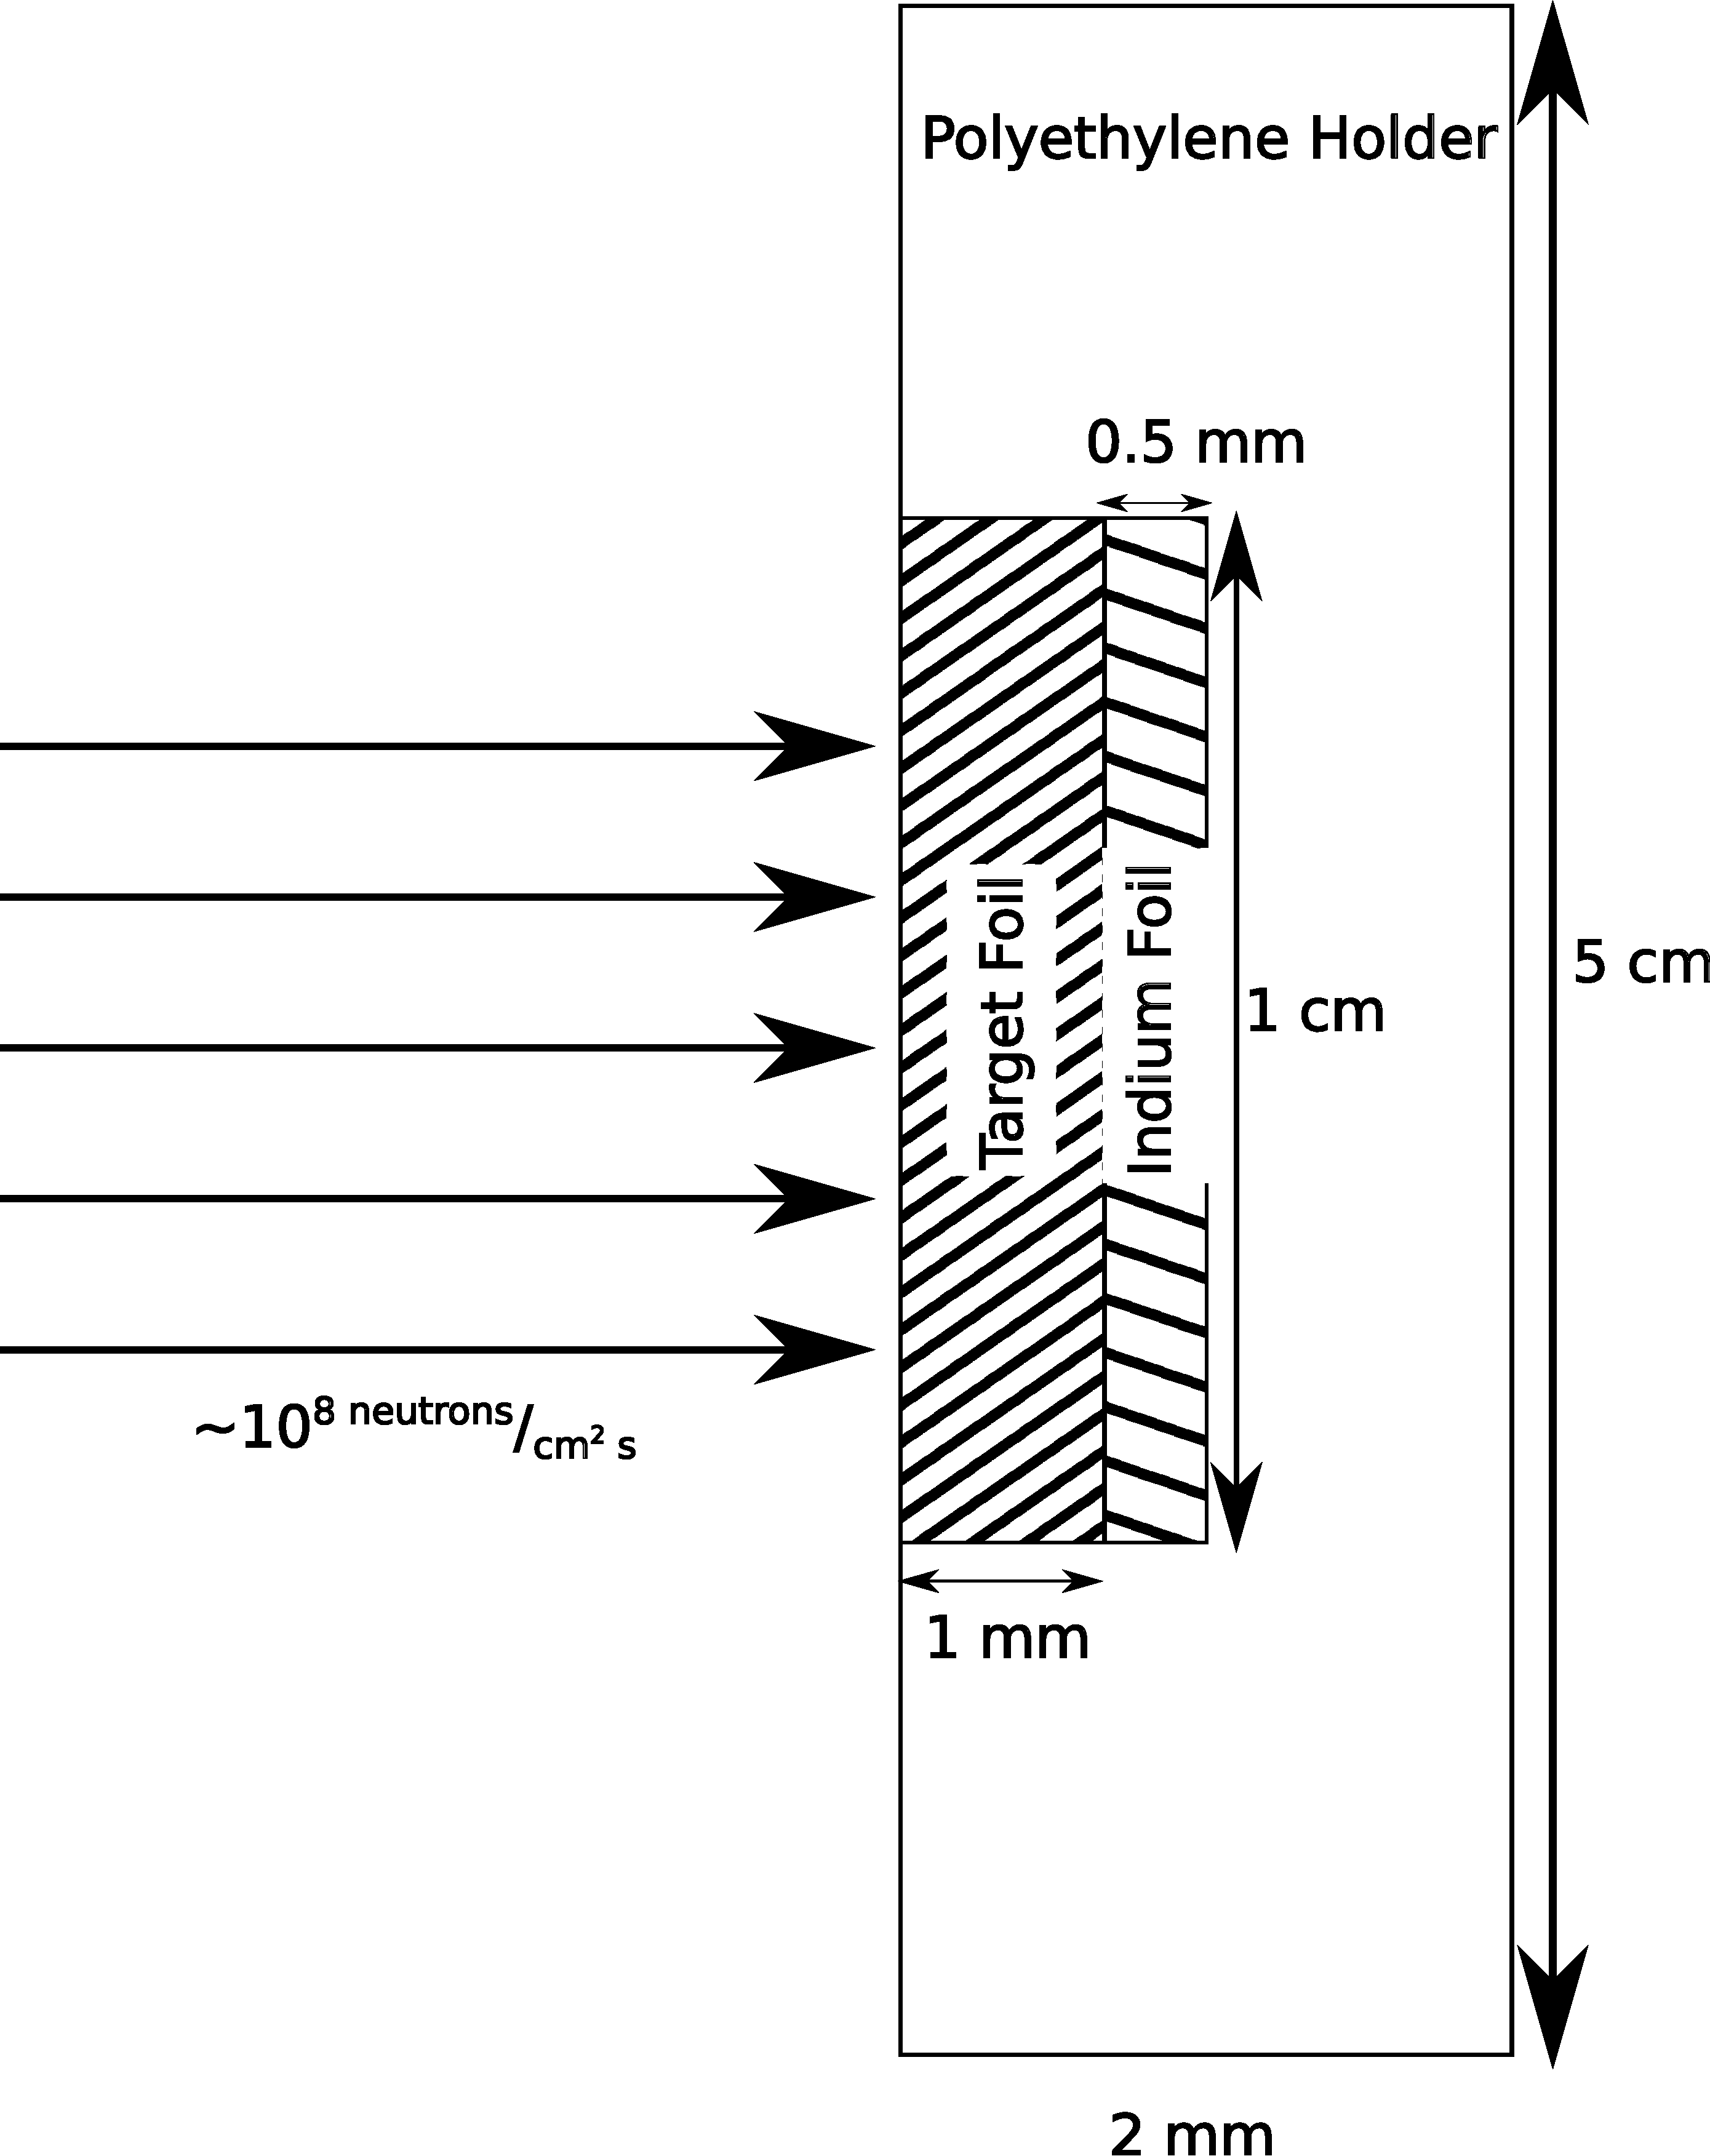
\includegraphics[height=2in]{./figures/holder.pdf}
        \caption{\color{red}{Use this or \autoref{fig:holder_a} - which is more appropriate?}}
                \label{fig:holder_b}
    \end{subfigure}
     ~ 
    \begin{subfigure}[t]{0.3\textwidth}
        \centering
%         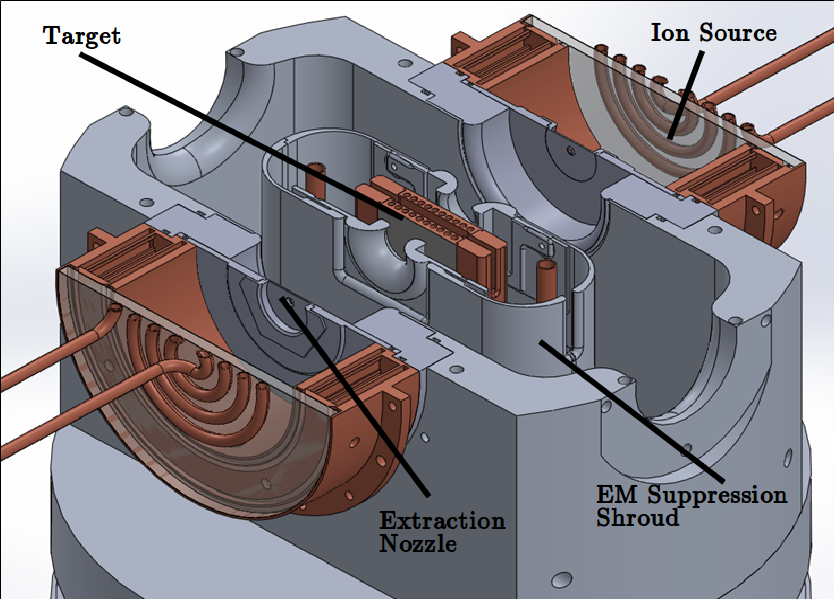
\includegraphics[width=\textwidth]{./figures/target2.png}
        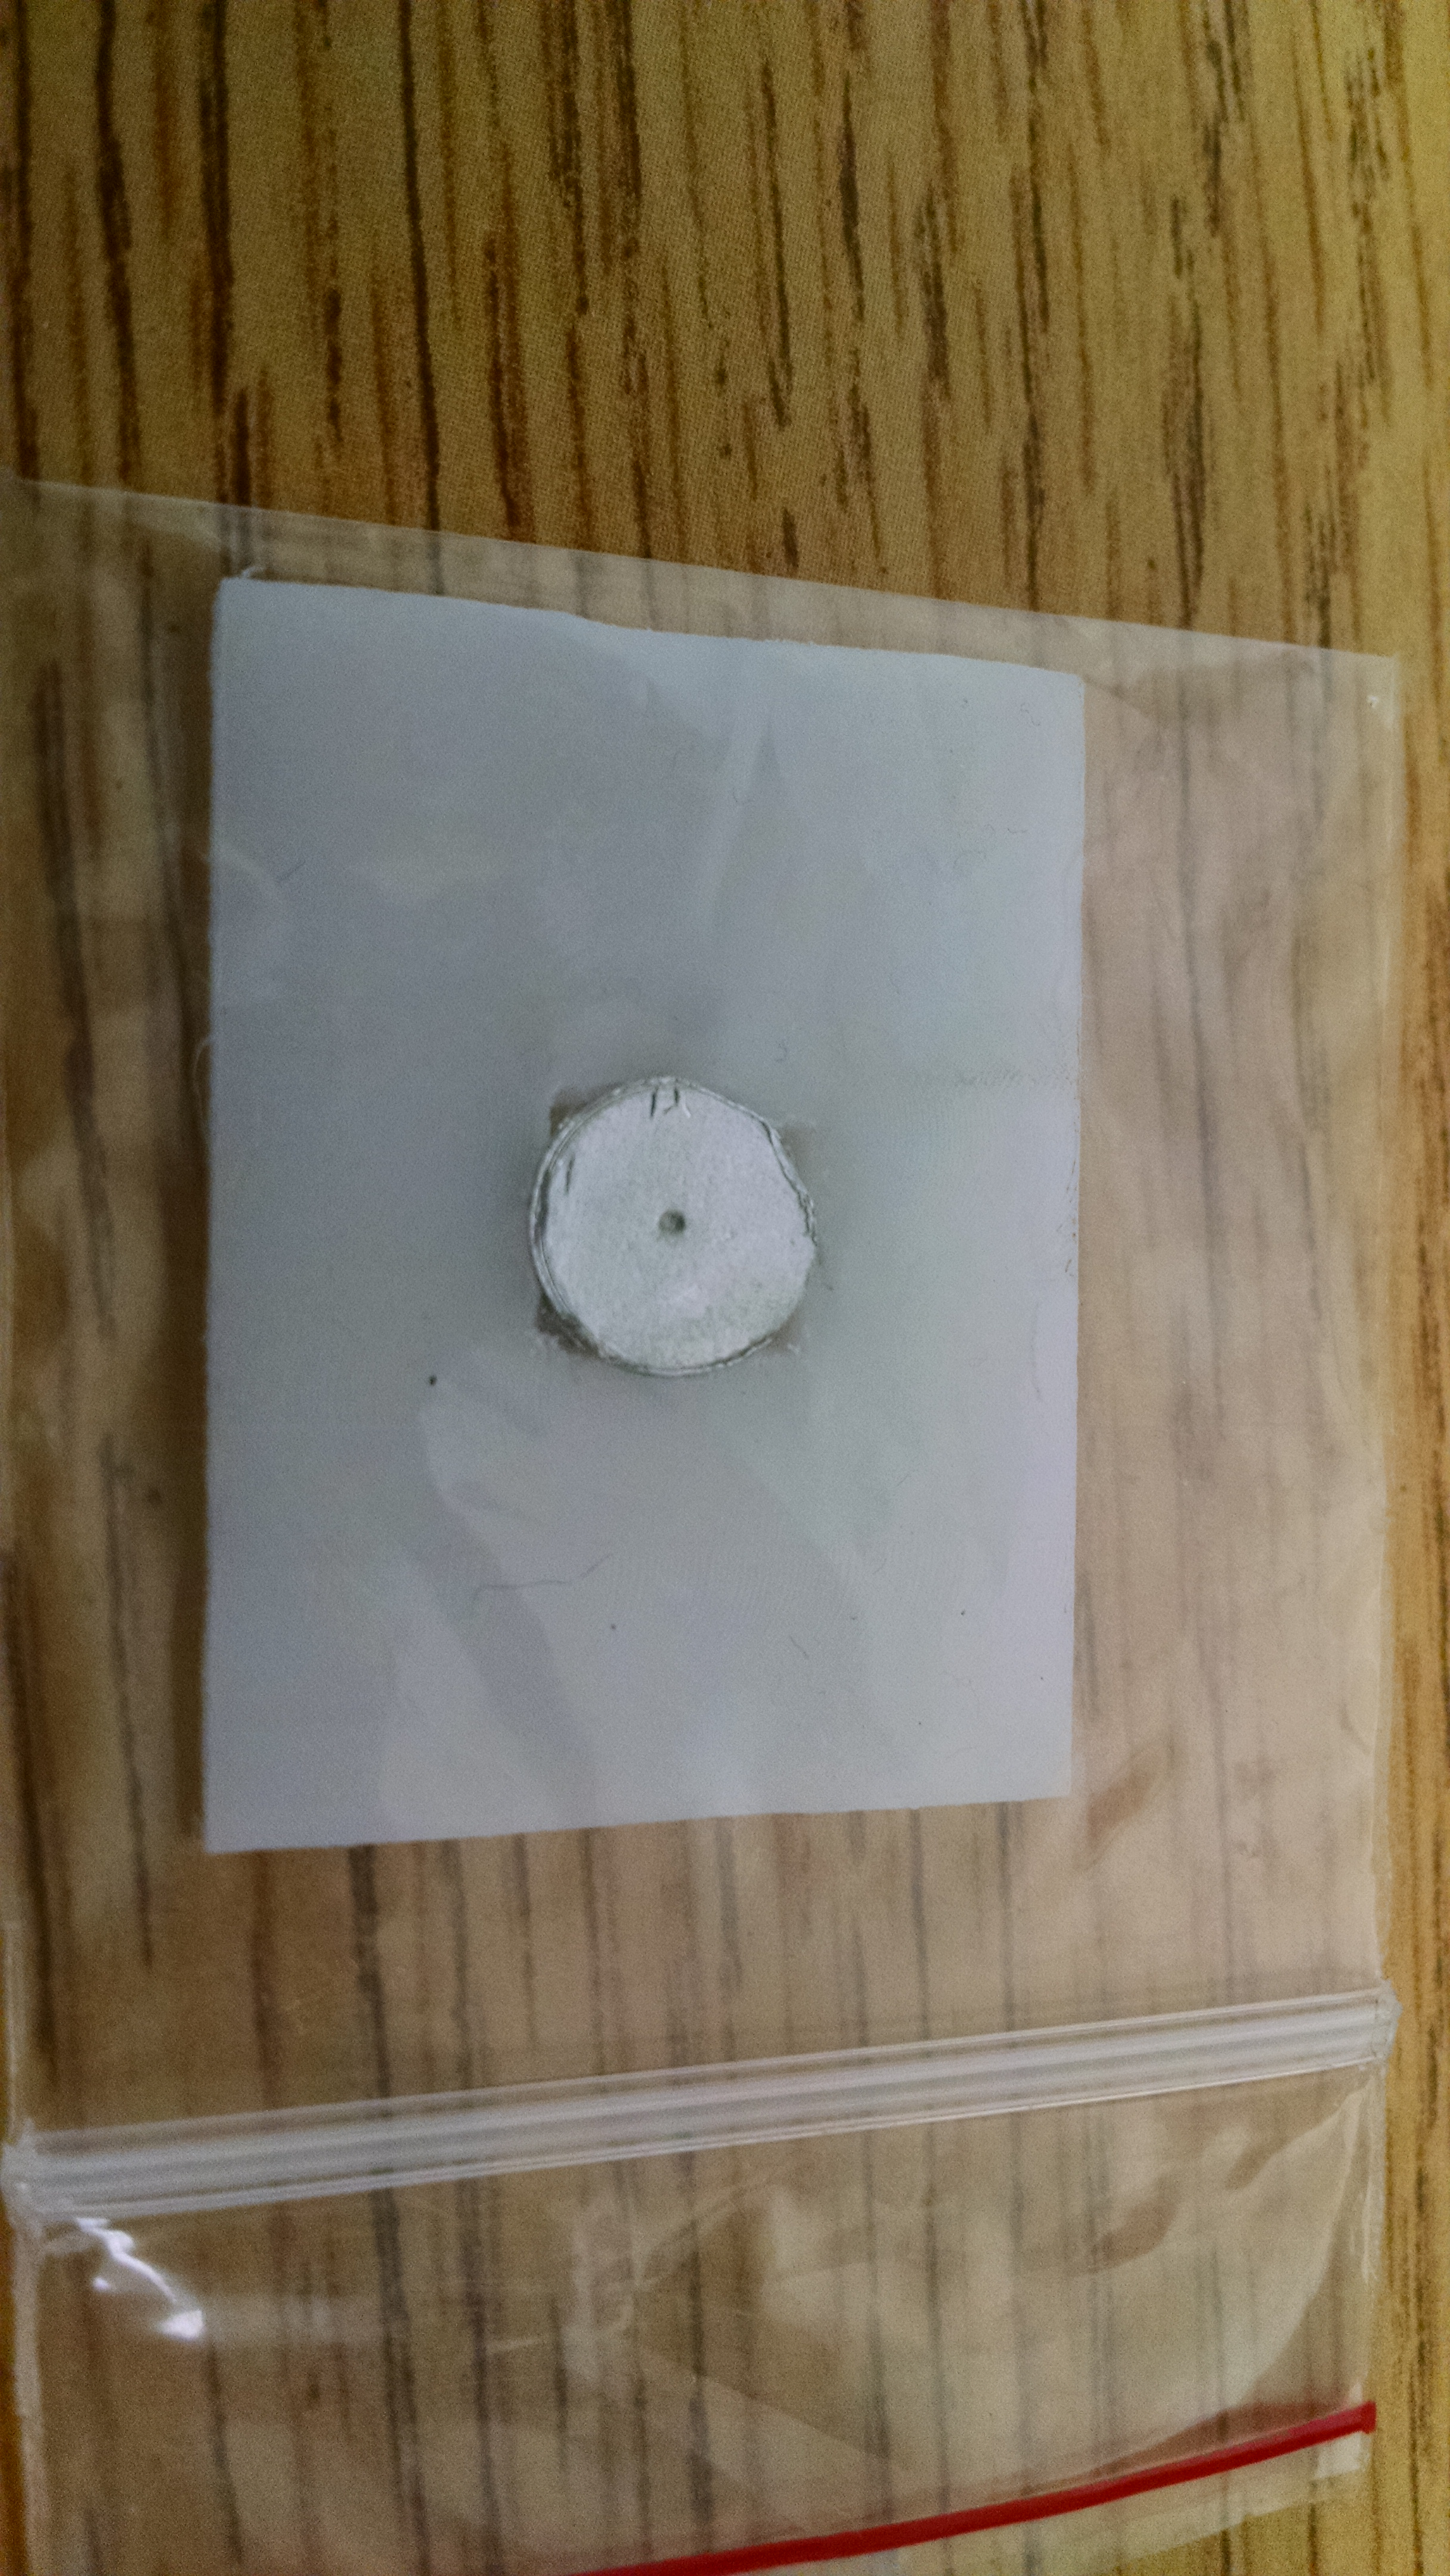
\includegraphics[height=2in]{./figures/IMG_20151103_113432563.jpg}
        \caption{ zinc (visible) foil co-loaded on top of reference indium foil, ready for irradiation.}
                \label{fig:holder_c}
    \end{subfigure}
    \caption{}
     \label{fig:main_holders}
\end{figure*}

For the measurement of the \ce{^{64}Zn}(n,p)\ce{^{64}Cu} cross section, a natural abundance commercial zinc foil of 1 cm diameter and 1 mm thickness was used as a target; a natural abundance titanium foil of the same dimensions was used as a target for the \ce{^{47}Ti}(n,p)\ce{^{47}Sc} reaction. For each run the target foils were co-loaded with a natural abundance Indium foil of 1 cm diameter and 0.5 mm thickness in a recess cut into a 2-mm thin polyethylene holder, as seen in \autoref{fig:main_holders}. Prior to loading, each foil was washed with isopropanol and dried, to remove any trace oils or residue that could become activated during irradiation.  \autoref{tab:foil_specs} records physical characteristics of each foil for the various irradiations. In each experiment, the co-loaded foils were irradiated for 3 hours at nominal operating conditions of 1.3 mA and 100 kV, to saturate the induced Indium isomer activity.

\comment{Regex to replace table hard link with LaTeX cross-reference.}

% Please add the following required packages to your document preamble:
% \usepackage{booktabs}
% \usepackage{graphicx}
\begin{table*}
\centering
\caption{Foil characteristics for each of the three (Zn/In)* experiments and the two (Ti/In)$^\dagger$  experiments. 
}
\label{tab:foil_specs}
\resizebox{\textwidth}{!}{%
\begin{tabular}{@{}ccccccc@{}}
\toprule
Foils Used & Metal Purity          & Abundance (a/o)                                                           & \begin{tabular}[c]{@{}c@{}}Foil Density \\ (mg/cm$^2$)\end{tabular} & Thickness (mm)                                                                                                         & Diameter (cm)                                                                                                           & Mass (g)                                                                                    \\ \midrule
$^\text{nat}$In      & \textgreater 99.999\% & \begin{tabular}[c]{@{}c@{}}\ce{^{113}In} (4.29\%),\\ \ce{^{115}In} (95.71\%)\end{tabular} & 365.5                                                            & \begin{tabular}[c]{@{}c@{}}0.49 $\pm$ 0.02*, \\ 0.50 $\pm$ 0.03*, \\ 0.49 $\pm$ 0.03*, \\ 0.53 $\pm$ 0.06$^\dagger$, \\ XXX $\pm$ XXX$^\dagger$\end{tabular} & \begin{tabular}[c]{@{}c@{}}9.75 $\pm$ 0.09*, \\ 9.98 $\pm$ 0.15*, \\ 9.96 $\pm$ 0.10*, \\ 10.01 $\pm$ 0.11$^\dagger$, \\ XXX $\pm$ XXX$^\dagger$\end{tabular} & \begin{tabular}[c]{@{}c@{}}0.248*, \\ 0.248*, \\ 0.241*, \\ 0.247$^\dagger$,\\  XXXXXX$^\dagger$\end{tabular} \\
$^\text{nat}$Zn      & \textgreater 99.99\%  & \ce{^{64}Zn} (49.17\%)                                                            & 714.1                                                            & \begin{tabular}[c]{@{}c@{}}1.03 $\pm$ 0.01, \\ 1.03 $\pm$ 0.01, \\ 1.02 $\pm$ 0.01\end{tabular}                                    & \begin{tabular}[c]{@{}c@{}}9.93 $\pm$ 0.14, \\ 9.76 $\pm$ 0.17, \\ 9.89 $\pm$ 0.15\end{tabular}                                     & \begin{tabular}[c]{@{}c@{}}0.538, \\ 0.451, \\ 0.452\end{tabular}                           \\
$^\text{nat}$Ti      & 99.999\%              & \ce{^{47}Ti} (7.44\%)                                                             & 450.6                                                            & \begin{tabular}[c]{@{}c@{}}1.16 $\pm$ 0.02, \\ XXXXXX\end{tabular}                                                         & \begin{tabular}[c]{@{}c@{}}9.93 $\pm$ 0.04, \\ XXXXXX\end{tabular}                                                          & \begin{tabular}[c]{@{}c@{}}0.337, \\ XXXXXXX\end{tabular}                                   \\ \bottomrule
\end{tabular}%
}
\end{table*}

\comment{Need foil data from Mauricio's 2nd Ti run}


\subsection{Determination of effective neutron energy}\label{sec:neutron_energies}

The kinematics of DD fusion at 100 keV lab energy produce neutrons of energy ranging from 2.2 to 2.85 MeV, over the lab-frame emission angular range of 0-180\degree, with respect to the incident deuteron beam. This distribution is a function of the incident deuteron kinetic energy, and has been well-documented \cite{Liskien_Paulsen_1973}; \autoref{fig:scatt_angle} displays the energy-angle distribution for the incident 100 keV deuterons used in the HFNG.

\comment{Parenthetical citations, or just a list at the end? The Shimizu paper uses the latter as citation format.}

\begin{figure}
 \centering
 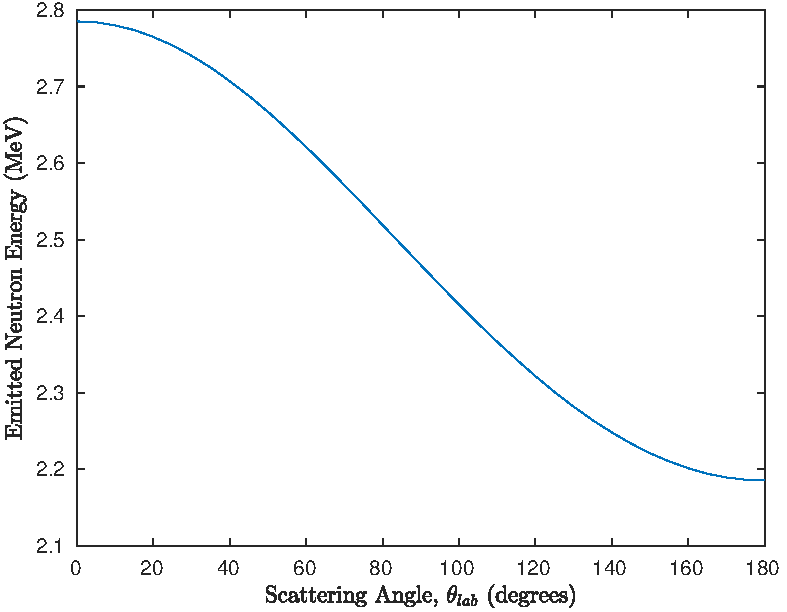
\includegraphics[scale=0.6]{./figures/scatt_angle.pdf}
 % scatt_angle.pdf: 369x295 pixel, 72dpi, 13.02x10.41 cm, bb=0 0 369 295
 \caption{Energy-angle distribution for neutrons emitted following DD fusion, for 100 keV incident deuterons.}
 \label{fig:scatt_angle}
\end{figure}

Collimated beamlines can be used to select an energy group from this distribution, by permitting only neutrons within a certain angular window to be incident upon a target. Due to the compact nature of the HFNG, this would require the mounting of samples outside of the target chamber, with a distance of at least 20 cm from the DD reaction surface. This would greatly reduce the flux (to approximately 10$^4$ neutrons/s\ cm$^2$ over 4$\pi$) subtended by a single target and require longer irradiations for activation, which exacerbates the effect of simultaneous production and decay in activation measurements. Instead, the samples are mounted internally in the HFNG target chamber, separated by 5 mm of copper from the DD reaction surface. This allows the samples to subtend a fairly narrow ($\sim$28\degree) angle of the forward-focused neutrons, while maintaining the high (approximately $\sci{1.3}{7}$neutrons/s\ cm$^2$ ) flux for activations. 

\comment{Make global flux / fluence unification}

\begin{figure}
 \centering
 %trim option's parameter order: left bottom right top
 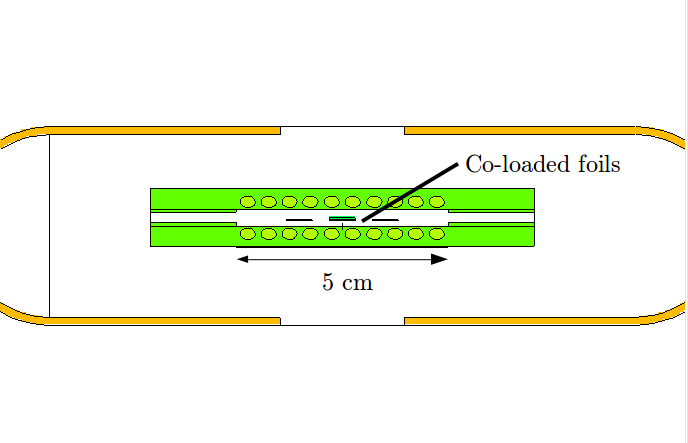
\includegraphics[trim = 0mm 0mm 2mm 0mm, clip,width=\columnwidth]{./figures/mcnp_vised2.png}
 % mcnp_vised2.PNG.png: 688x443 pixel, 96dpi, 18.21x11.72 cm, bb=0 0 516 332
 \caption{MCNP6 model of the Berkeley HFNG target chamber, with reference scale. The co-loaded foils can be seen in the target chamber center.}
 \label{fig:mcnp_vised}
\end{figure}

\comment{Need to replace this figure - coming from Mauricio?}

To determine the energy distribution of neutrons incident upon the loaded foils following production and transport, the Monte Carlo N-Particle transport code  MCNP6 \cite{goorley2013initial} was used to model the neutron energy spectrum incident upon target foils co-loaded into the HFNG (see \autoref{fig:mcnp_flux}). This spectrum illustrates the forward-focused kinematics of the DD reaction subtended by the co-loaded sample foils.

% \begin{figure}
%  \centering
%  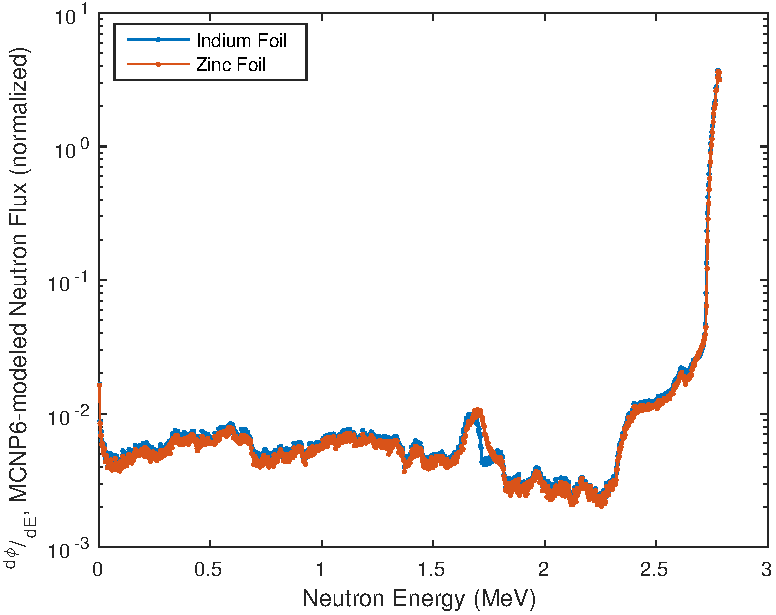
\includegraphics[scale=0.6]{./figures/mcnp_flux.pdf}
%  % mcnp_flux.pdf: 373x295 pixel, 72dpi, 13.16x10.41 cm, bb=0 0 373 295
%  \caption{MCNP6-modeled neutron energy spectrum for the Berkeley HFNG, using co-loaded indium and zinc (for \ce{^{64}Cu} production) foils as an example.}
%  \label{fig:mcnp_flux}
% \end{figure}

\begin{figure}
 \centering
 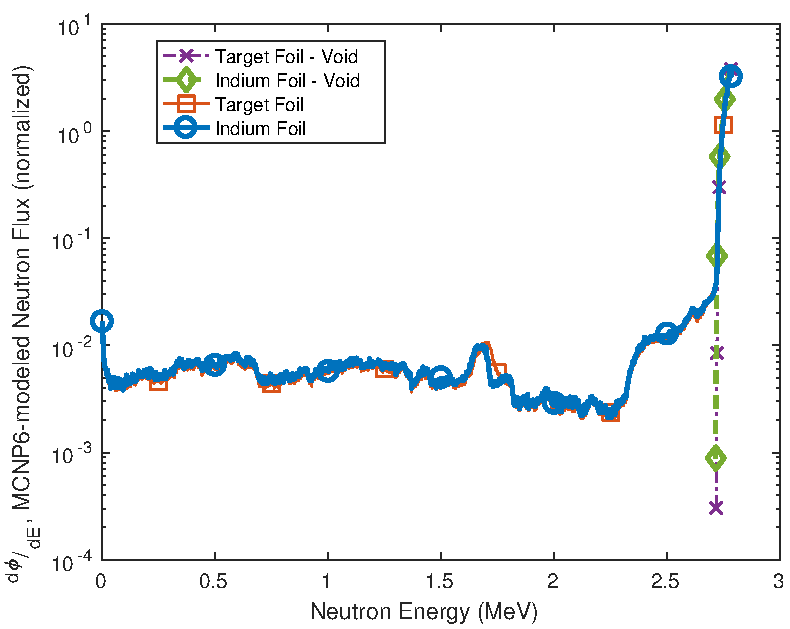
\includegraphics[scale=0.6]{./figures/mcnp_flux_new.pdf}
 % mcnp_flux.pdf: 373x295 pixel, 72dpi, 13.16x10.41 cm, bb=0 0 373 295
 \caption{MCNP6-modeled neutron energy spectrum for the Berkeley HFNG, using co-loaded indium and zinc (for \ce{^{64}Cu} production) foils as an example.}
 \label{fig:mcnp_flux}
\end{figure}


\comment{Use this version, old version (mcnp-flux.pdf), or some new combination of lines?}

While this shows that the sample foils receive a very narrow energy distribution of incident neutrons, an effective neutron energy and energy bounds must be determined to constrain cross section ratio measurements. From the same MCNP6 simulation, flux tallies show a flux-weighted average neutron energy of 2.7645 MeV in the Indium foil, and 2.7649 MeV in the zinc or titanium foil; these are indistinguishable within statistical uncertainty, and serve as an effective neutron energy in the loaded target foils. Due to the kinematics of DD neutron emission, $E_{max}$,  the maximum energy of a neutron subtending the target foils in this geometry is 2.7825 MeV. For this maximum energy, the number of reactions induced in a foil (containing $N_i$ target nuclei) is simply:

\begin{equation}
R = N_i \int_0^{E_{max}} \sigma(E) \dfrac{d\phi}{dE} dE
\end{equation}


\comment{Regex to replace equations with LaTeX formats, add cross-references.}

From this definition, it is possible to calculate $F\pp{E'}$, the fraction of total reactions induced up to some energy $E' < E_{max}$:

\begin{equation}\label{eqn:react_fraction}
F\pp{E'} = \dfrac{\int_0^{E'} \sigma(E) \dfrac{d\phi}{dE} dE}{\int_0^{E_{max}} \sigma(E) \dfrac{d\phi}{dE} dE}
\end{equation}

% \begin{figure}
%  \centering
%  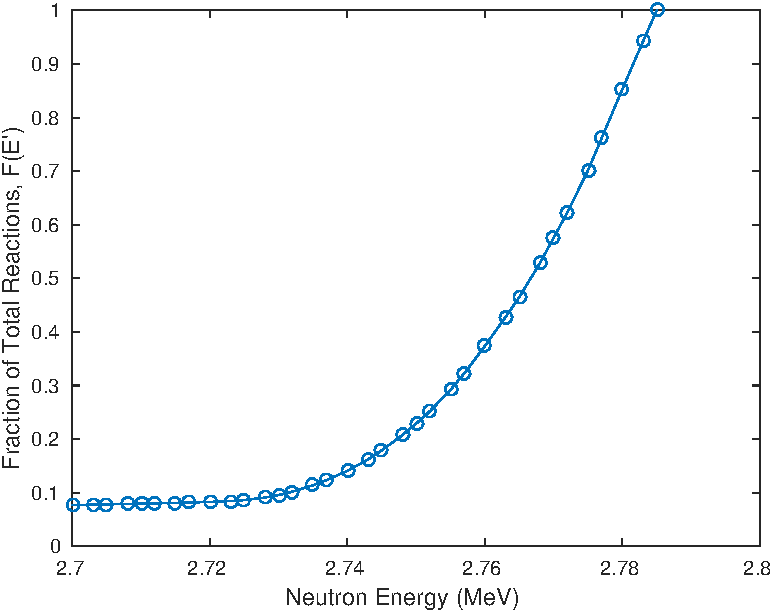
\includegraphics[scale=0.6]{./figures/fracplot.pdf}
%  % fracplot.pdf: 372x295 pixel, 72dpi, 13.12x10.41 cm, bb=0 0 372 295
%  \caption{Fraction of total reactions induced in the Indium foil between the energies [0, $E'$]}
%  \label{fig:frac_plot}
% \end{figure}

\begin{figure}
 \centering
 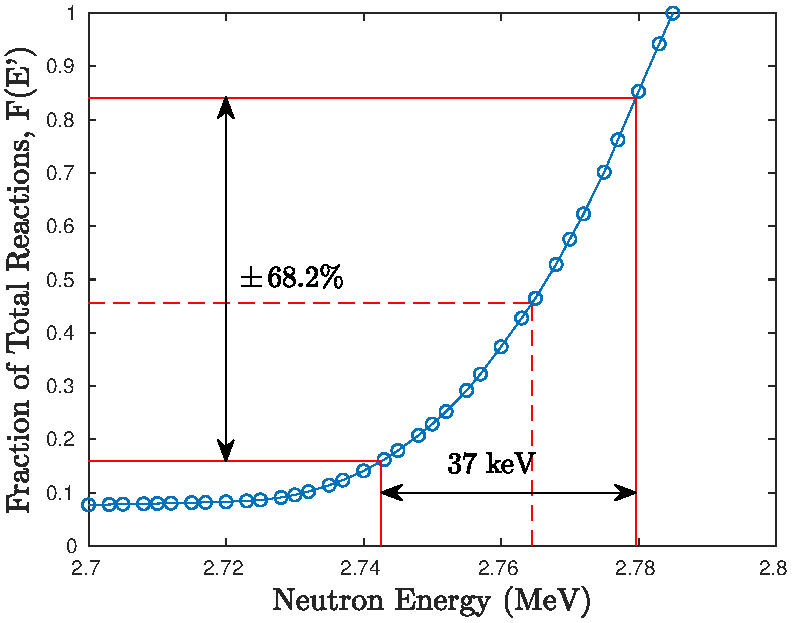
\includegraphics[scale=0.6]{./figures/fracplot_new.pdf}
 % fracplot.pdf: 372x295 pixel, 72dpi, 13.12x10.41 cm, bb=0 0 372 295
 \caption{Fraction of total reactions induced in the Indium foil between the energies [0, $E'$]}
 \label{fig:frac_plot}
\end{figure}

\comment{Use this version, or old version (fracplot.pdf)?}



This quantity $F\pp{E'}$ is plotted in \autoref{fig:frac_plot}. Using the flux-averaged neutron energy in the Indium foil as a centroid, this fraction of total reactions can be used to estimate the uncertainty in effective neutron energy, which will become energy error bars in the excitation function for these reactions. Within 1 standard deviation above and below the centroid, 68.2\% of all reactions should be encompassed. Thus, the upper and lower energy uncertainties correspond to the neutron energies $E'$  such that $F\pp{E'}$ = 0.841 and $F\pp{E'}$ = 0.159, respectively. From \autoref{eqn:react_fraction},  these are found to be  F(2.7796 MeV) = 0.841 and F(2.7426 MeV) = 0.159, respectively; thus the effective neutron energy subtended by target foils is reported as $E_n$ = 2.7645 MeV + 0.0151 MeV / - 0.0219 MeV.  This 37-keV full-energy spread verifies that, at such close distances to the DD reaction surface, loaded target foils receive a highly quasi-monoenergetic neutron flux.





\subsection{Measurement of induced activities}\label{sec:spectroscopy}

After irradiation, the co-loaded targets in each experiment were removed from the HFNG and transferred to a counting lab, where their induced activities could be measured via gamma ray spectroscopy. Two detectors were used in this measurement: an Ortec 80\% High-Purity Germanium (HPGe) detector (calibrated from 50 keV - 3800 keV) used for the detection of the higher-energy gamma rays in the \ce{^{64}Zn}(n,p)\ce{^{64}Cu} experiments, and an Ortec planar Low-Energy Photon Spectrometer (LEPS) detector (calibrated from 15 keV - 450 keV) used for the detection of the lower-energy gamma rays in the \ce{^{47}Ti}(n,p)\ce{^{47}Sc} experiments. These can be seen in \autoref{fig:hpge_a} and \autoref{fig:hpge_b}. Both detectors were calibrated for both energy and efficiency, using \ce{^{133}Ba}, \ce{^{137}Cs}, and \ce{^{152}Eu} sources at various distances from the front face of each detector. These efficiencies, along with gamma ray intensities for each transition, are used to convert the integrated counts in each gamma ray photopeak into an activity for the activated isotopes and isomeric states. 


\begin{figure*}[H]
    \centering
    \begin{subfigure}[t]{0.7\textwidth}
        \centering
%         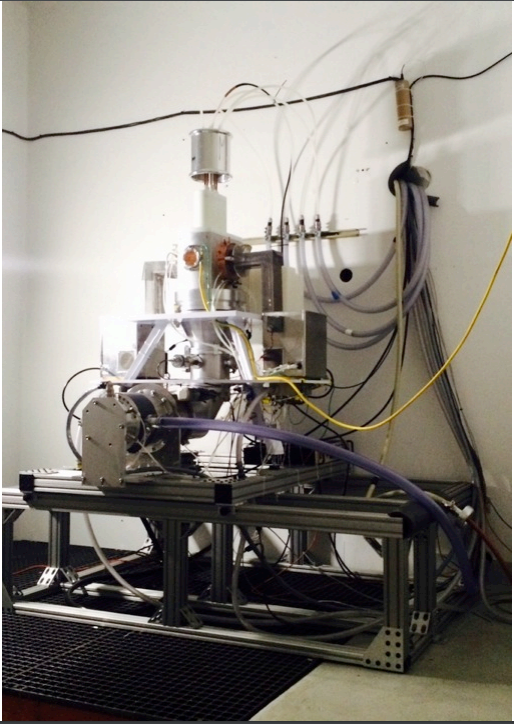
\includegraphics[width=\columnwidth]{./figures/Capture.PNG}
        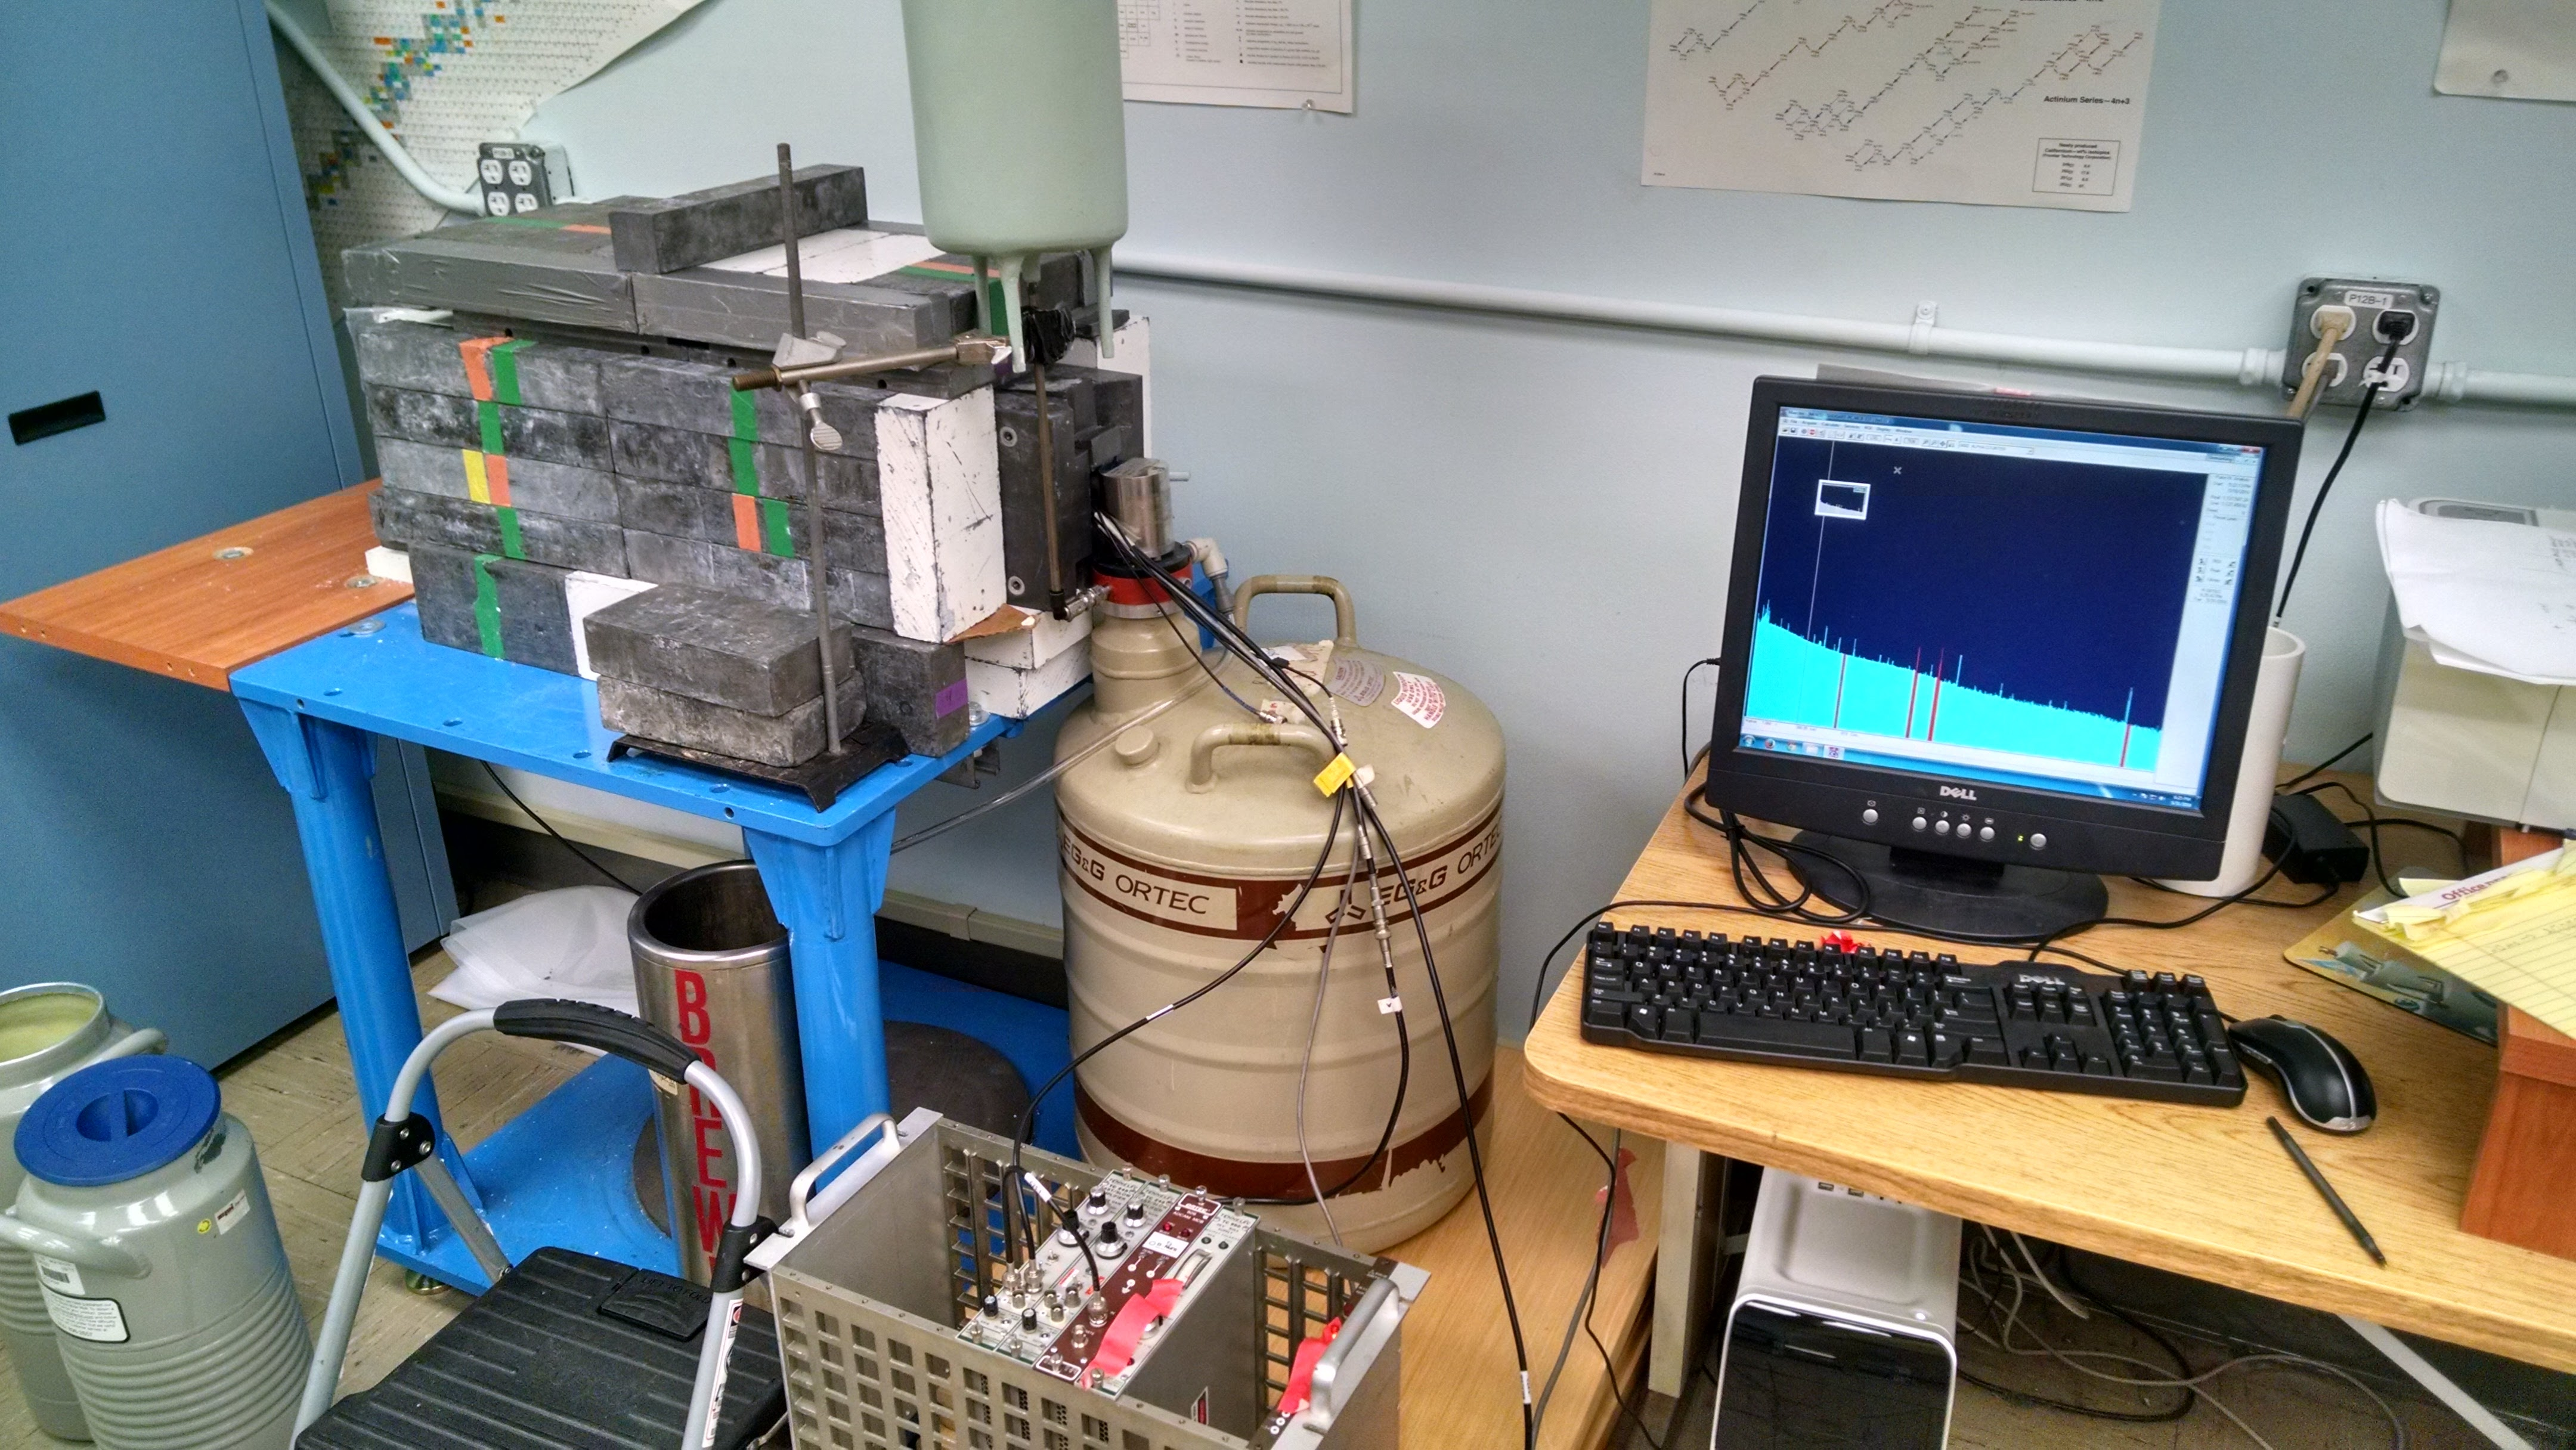
\includegraphics[height=2.8in]{./figures/IMG_20160531_182618557_HDR.jpg}
        \caption{ Ortec 80\% HPGe detector}
        \label{fig:hpge_a}
    \end{subfigure}%
    ~ 
    \begin{subfigure}[t]{0.28\textwidth}
        \centering
%         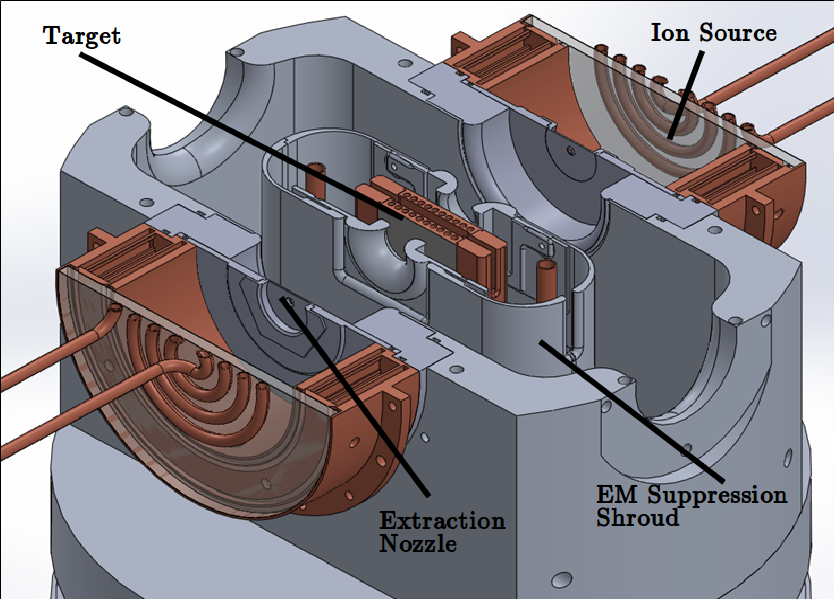
\includegraphics[width=\textwidth]{./figures/target2.png}
        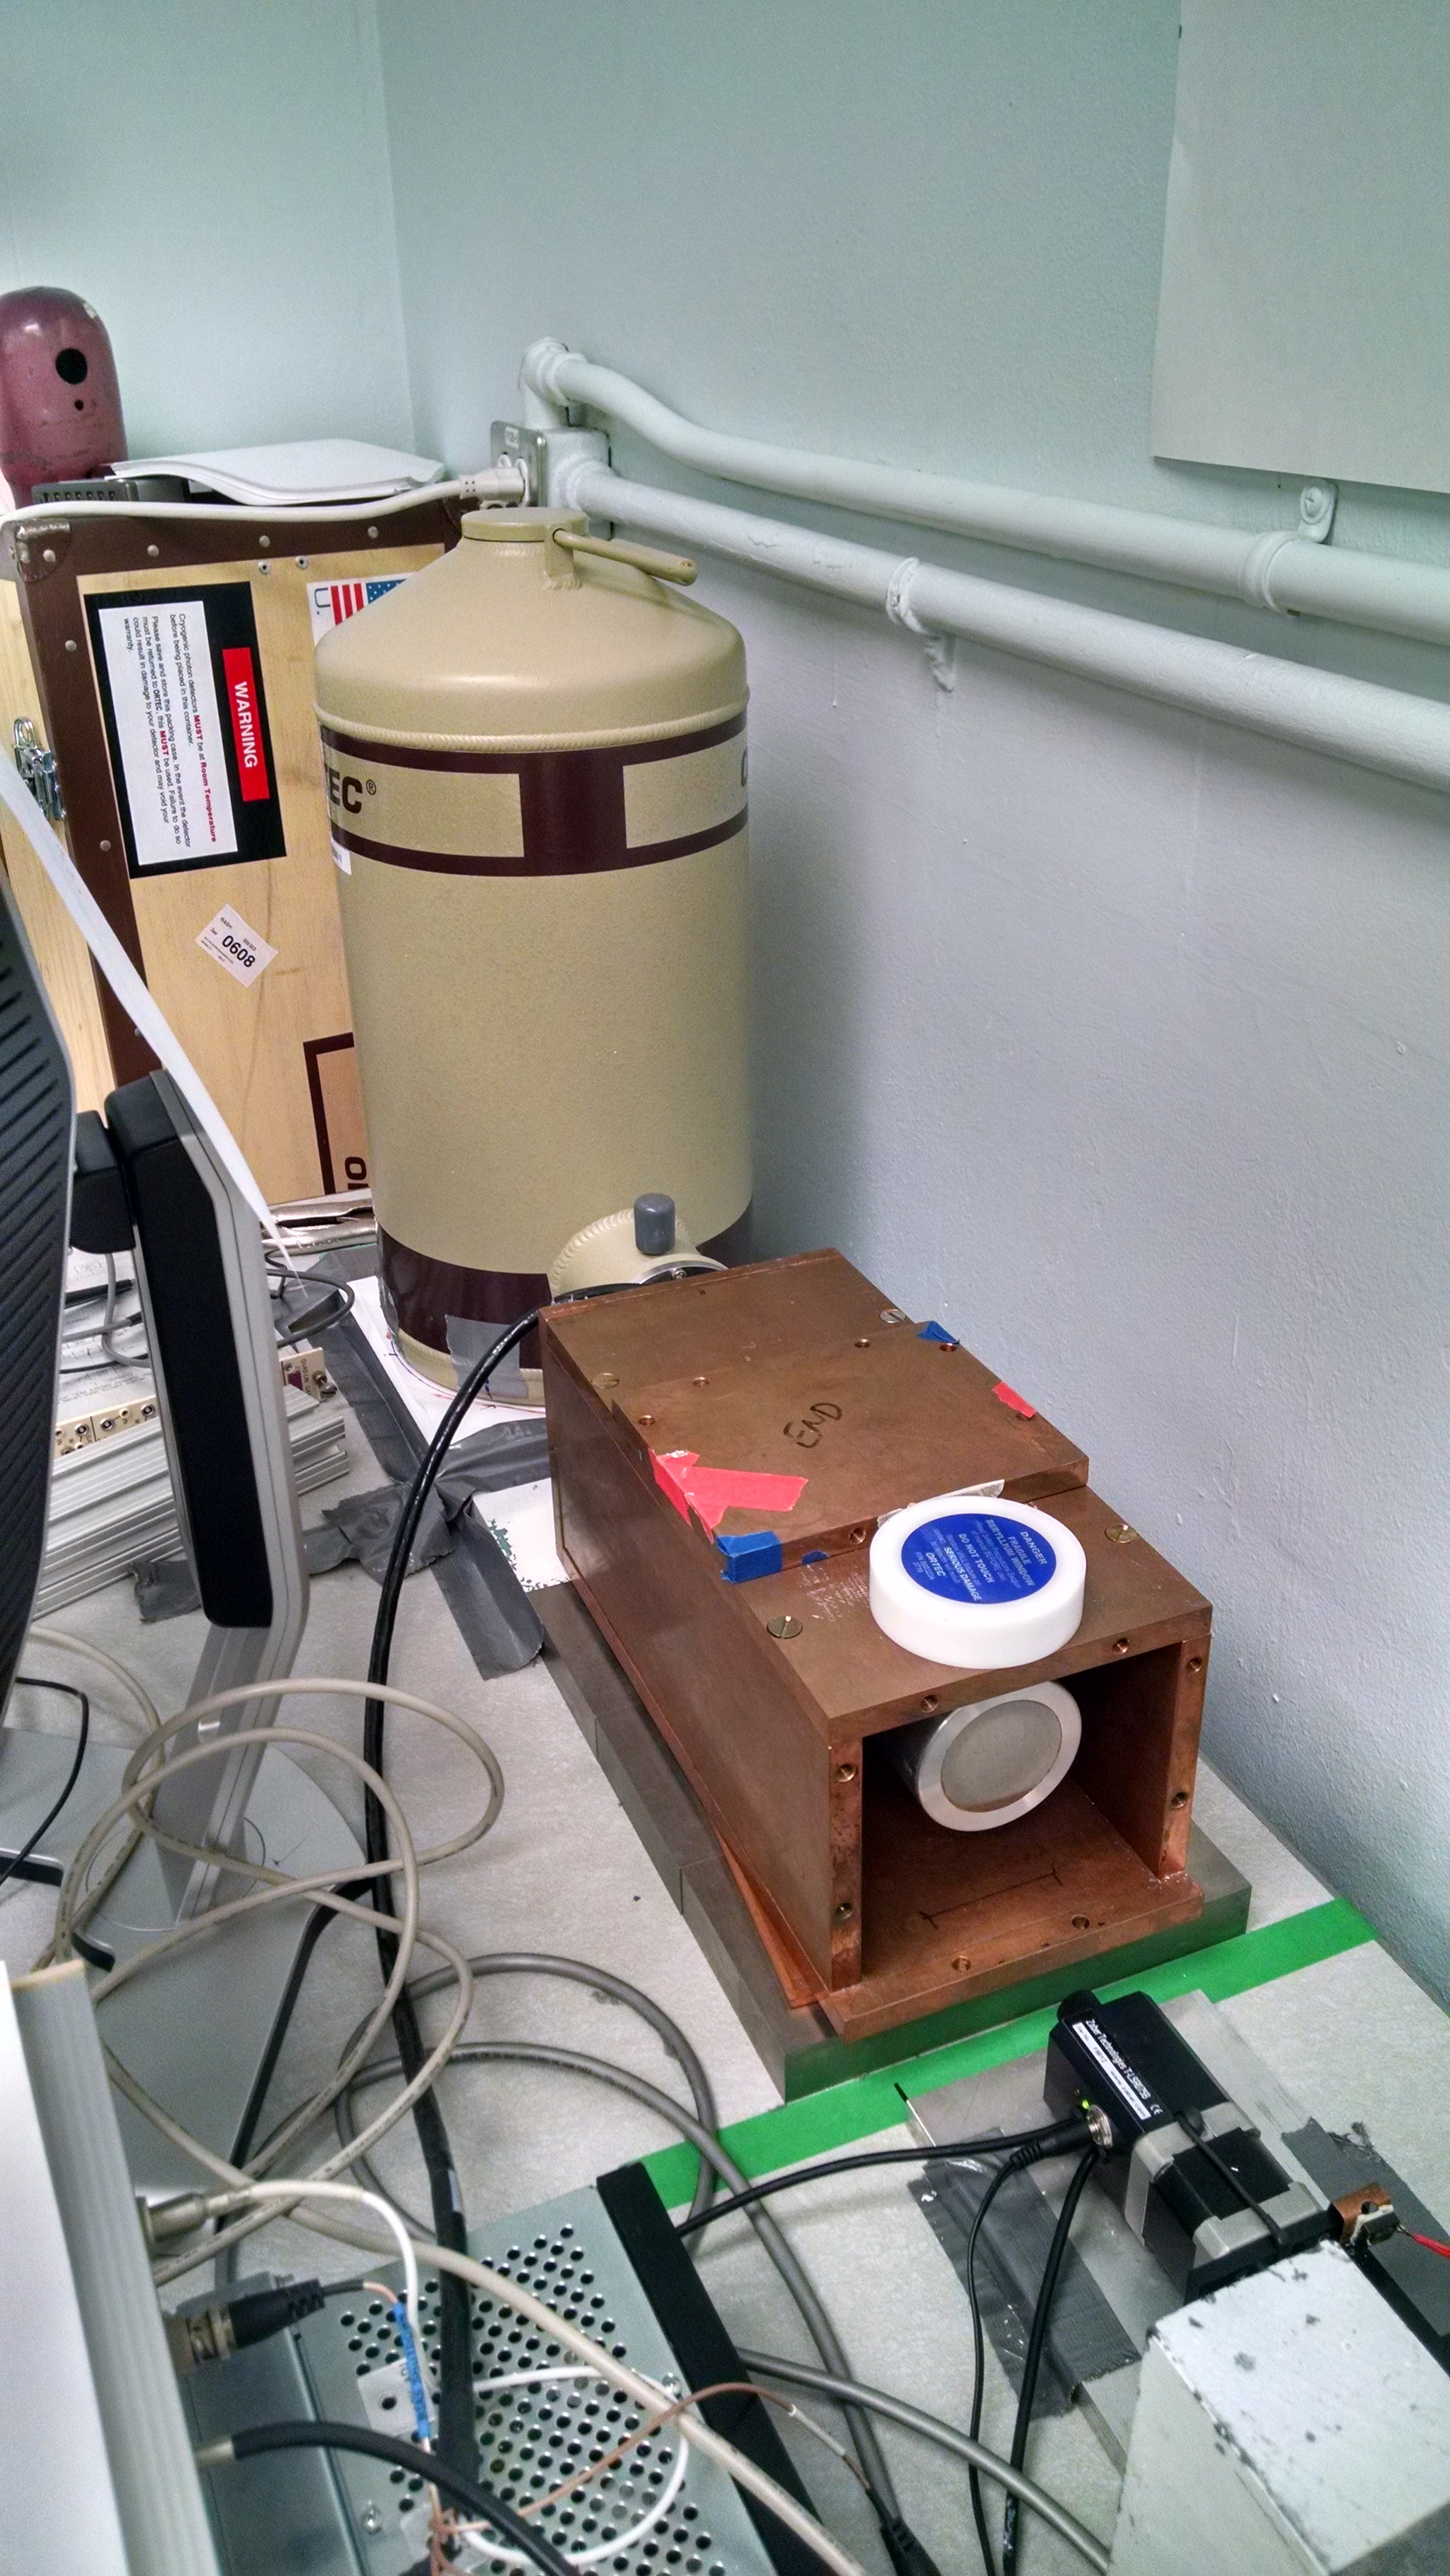
\includegraphics[height=2.8in]{./figures/IMG_20160531_182635712_HDR.jpg}
        \caption{Ortec planar LEPS detector}
                \label{fig:hpge_b}
    \end{subfigure}
    \caption{High-Purity Germanium Detectors used for gamma spectroscopy of the activated foils.}
     \label{fig:main_ge_detectors}
\end{figure*}

\comment{Does \autoref{fig:main_ge_detectors} serve any purpose? Should it be cut?}

The foils were counted in their polyethylene holder, and placed close to the front face of the detector in use, with the target foil (zinc or titanium) facing towards the front face of the detector when both target and monitor foils were counted simultaneously. This position allows for the detectors to subtend the largest possible solid angle of the gamma rays emitted by the foils. All data collection was performed using the Ortec MAESTRO software. For each experiment the detector dead time was verified to be less than 5\%, to avoid coincidence summing effects. This was never an issue for any experiments, but had it been, the foils would be moved to a position of greater standoff from the detector, to reduce the dead time.  For the  \ce{^{47}Sc} production experiments, the foils were counted simultaneously using a planar LEPS detector. For the \ce{^{64}Cu} production experiments, the Indium foil was first counted separately using an 80\% HPGe detector, to capture the short-lived Indium activities. This is due to the fact that the \ce{^{115}In} can undergo the \ce{^{115}In}(n,$\gamma$)\ce{^{116}In} reaction, with a cross section of 83 mb for 2.76 MeV neutrons. \ce{^{116}In} has a 54 minute half-life, decaying via $\beta^-$ with a Q value of 3.278 MeV. This decay populates several states in \ce{^{116}Sn} capable of emitting gamma rays with $E_\gamma > 2 \times$ the 511-keV gamma, which is produced via pair production in the detector crystal, contaminating the 511-keV channel used to monitor  \ce{^{64}Cu} production. After approximately 4 hours of spectra collection, the activated zinc foil was added back and counting resumed simultaneously with the indium foil. This allowed for decay of nearly all \ce{^{116}In}, avoiding significant 511 keV contamination. Example spectra for each production pathway can be seen in \autoref{fig:spectra_a} and \autoref{fig:spectra_b}.


\begin{figure*}[H]
    \centering
    \begin{subfigure}[t]{\textwidth}
        \centering
%         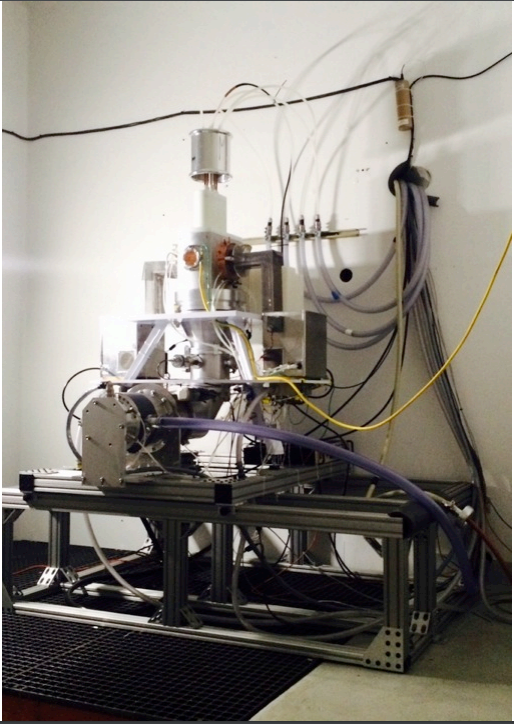
\includegraphics[width=\columnwidth]{./figures/Capture.PNG}
%         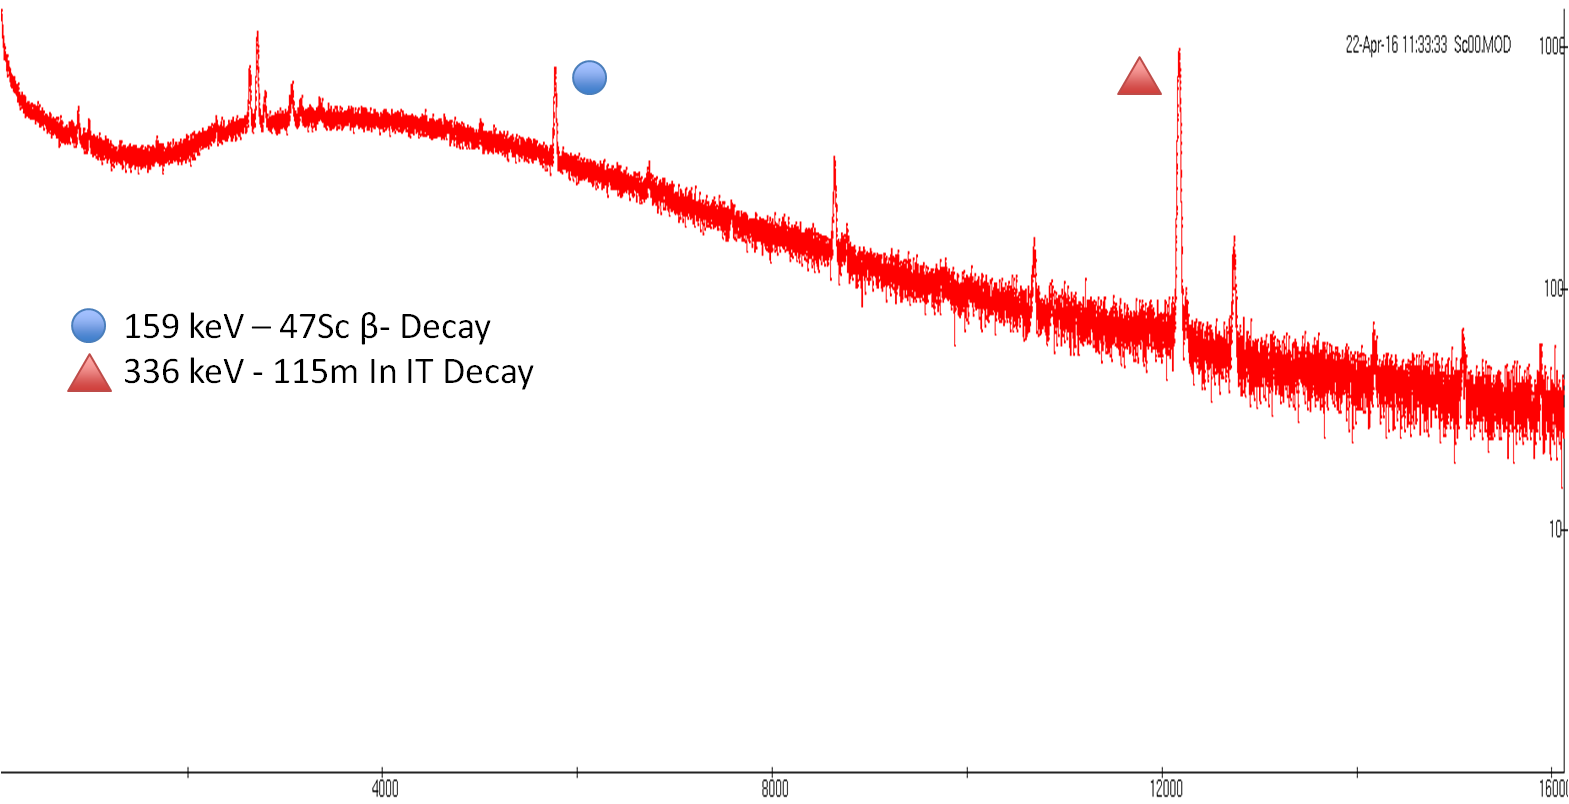
\includegraphics[width=5in]{./figures/ti_foils.png}
        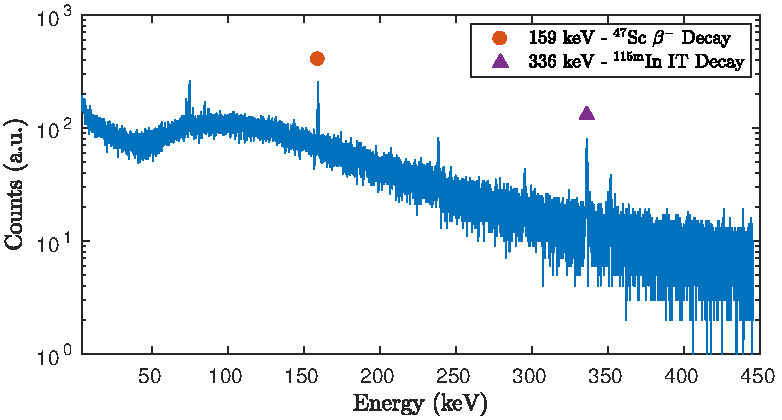
\includegraphics[width=5in]{./figures/47sc_gspectrum_alt.pdf}
        \caption{ Gamma spectrum for the \ce{^{47}Ti}(n,p)\ce{^{47}Sc} production pathway foils, counted using a planar LEPS detector}
        \label{fig:spectra_a}
    \end{subfigure}%
    \\
    \begin{subfigure}[t]{\textwidth}
        \centering
%         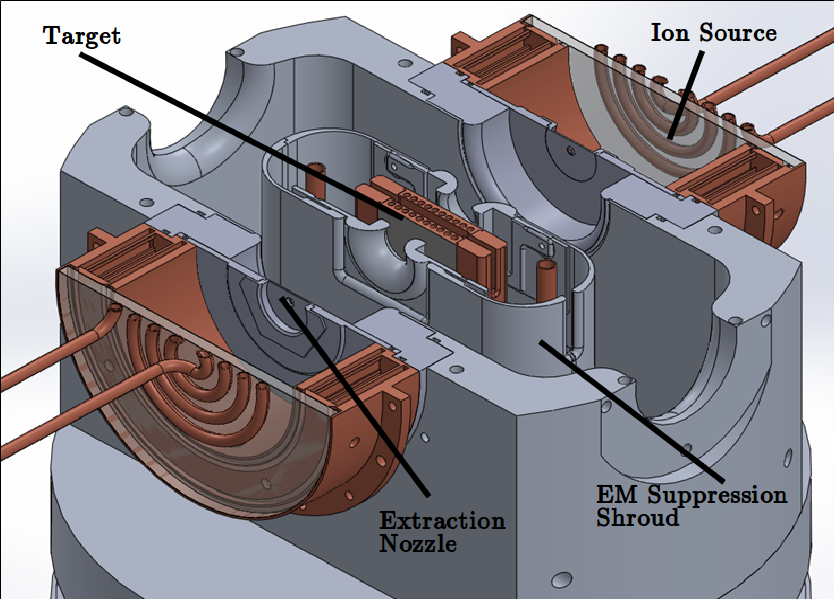
\includegraphics[width=\textwidth]{./figures/target2.png}
%         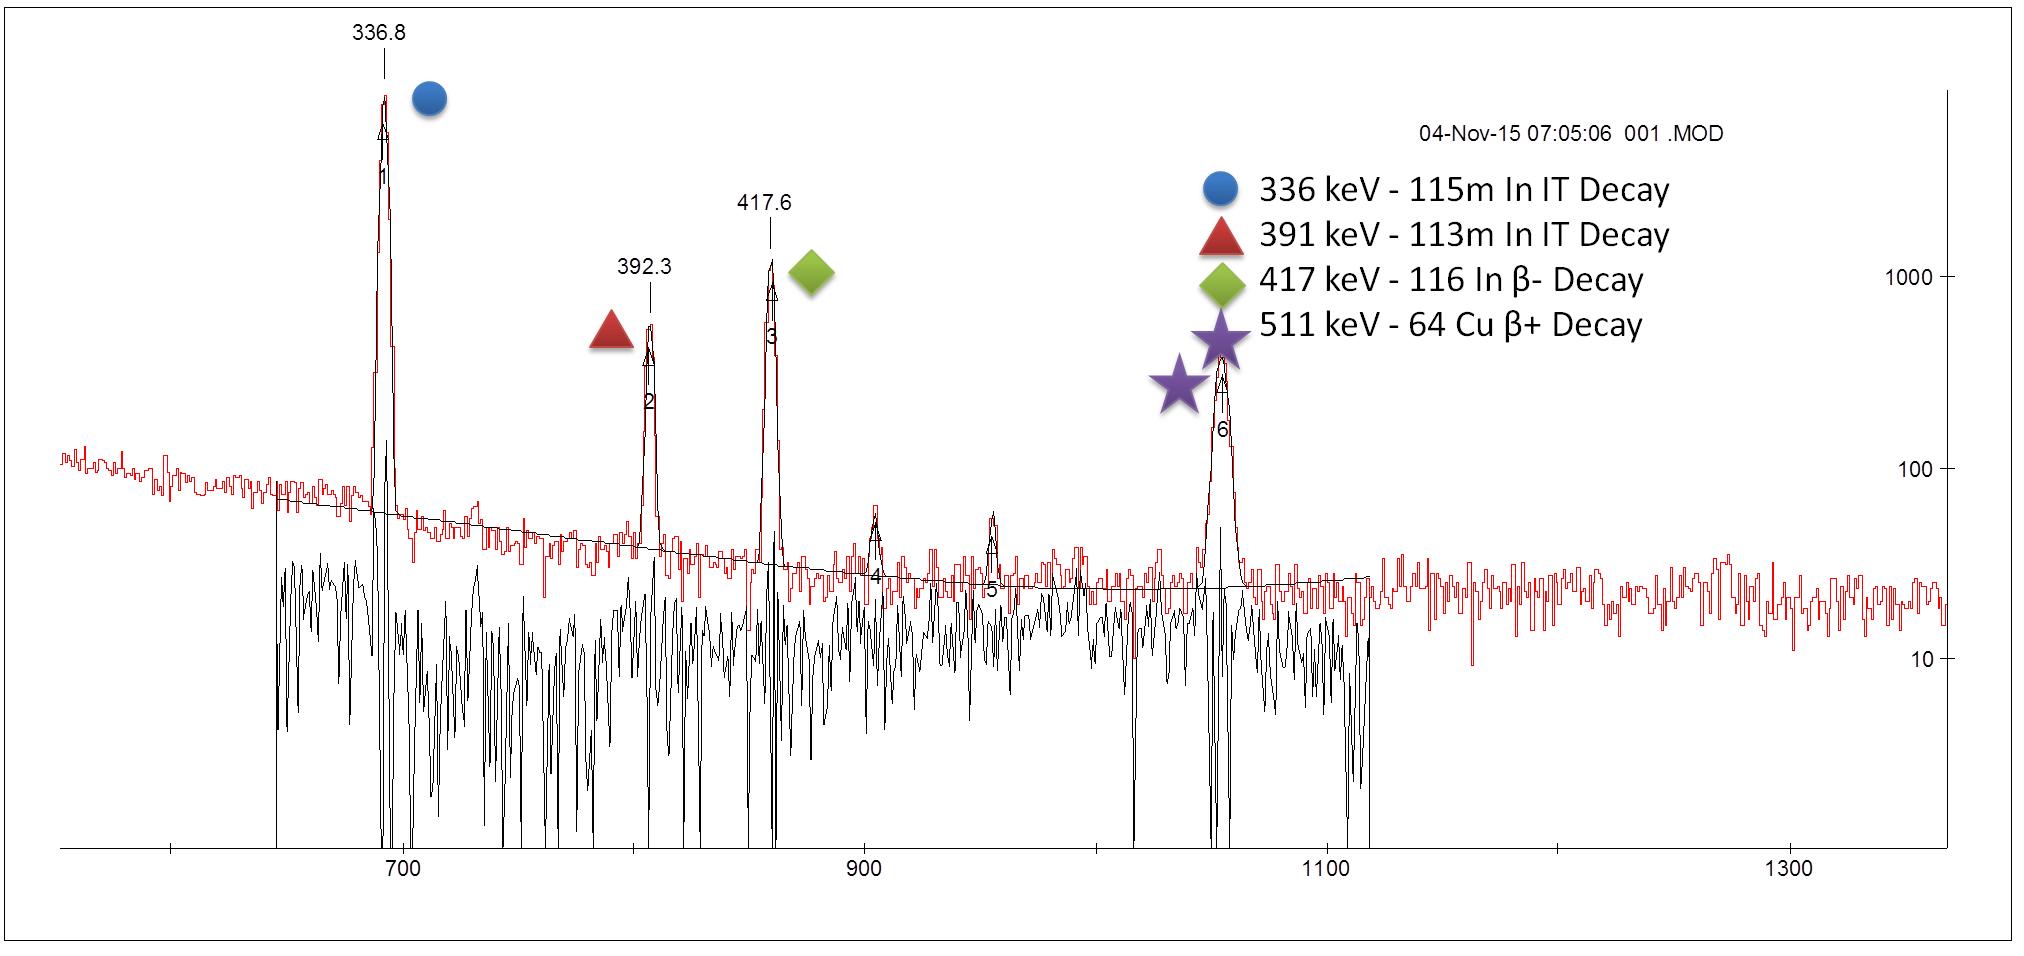
\includegraphics[width=5in]{./figures/Sample_spectra.png}
        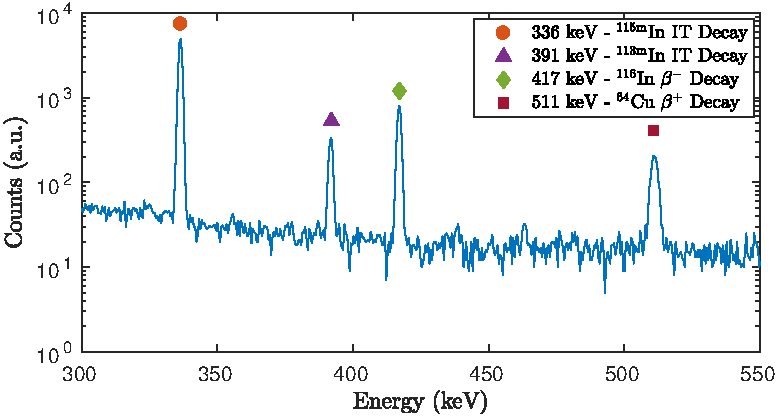
\includegraphics[width=5in]{./figures/64Cu_gspectrum_alt.pdf}
        \caption{Gamma spectrum for the \ce{^{64}Zn}(n,p)\ce{^{64}Cu} production pathway foils, counted using an 80\% HPGe detector.}
                \label{fig:spectra_b}
    \end{subfigure}
    \caption{Example gamma spectra collected to monitor radioisotope production.}
     \label{fig:main_spectra}
\end{figure*}

\comment{Example spectra are messy - being updated...}

To verify that each peak corresponds to the assigned transitions, spectra were acquired in a sequence of 15 - 30 minute intervals. By plotting the background-subtracted photopeak counts for a particular channel as a function of time, an exponential decay function may be fit to it, to determine the half-life of the transition in question. Plots of these curves for each transition in this work are seen in Figures \ref{fig:decay_curve_336} - \ref{fig:decay_curve_511}. The fitted functions for each transition agree (at the 1$\sigma$ confidence level) with accepted half-lives from the ENSDF library, confirming the respective peak assignments.

\comment{Reference original ENSDF papers?}

\begin{figure*}
    \centering
    \begin{subfigure}[t]{0.49\textwidth}
        \centering
%         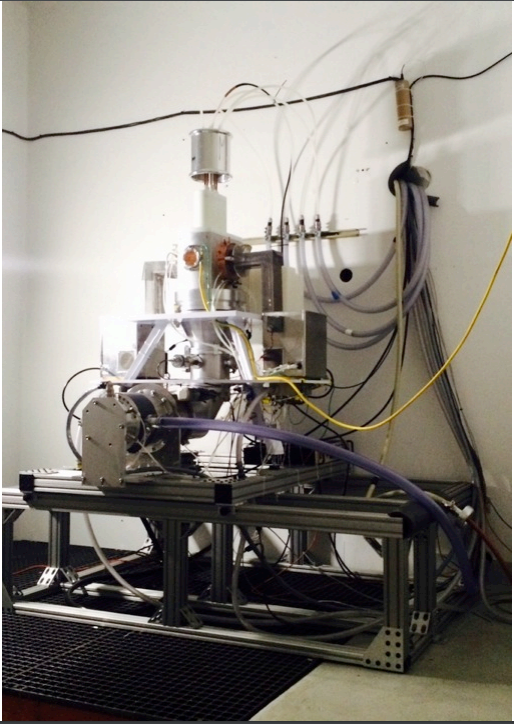
\includegraphics[width=\columnwidth]{./figures/Capture.PNG}
        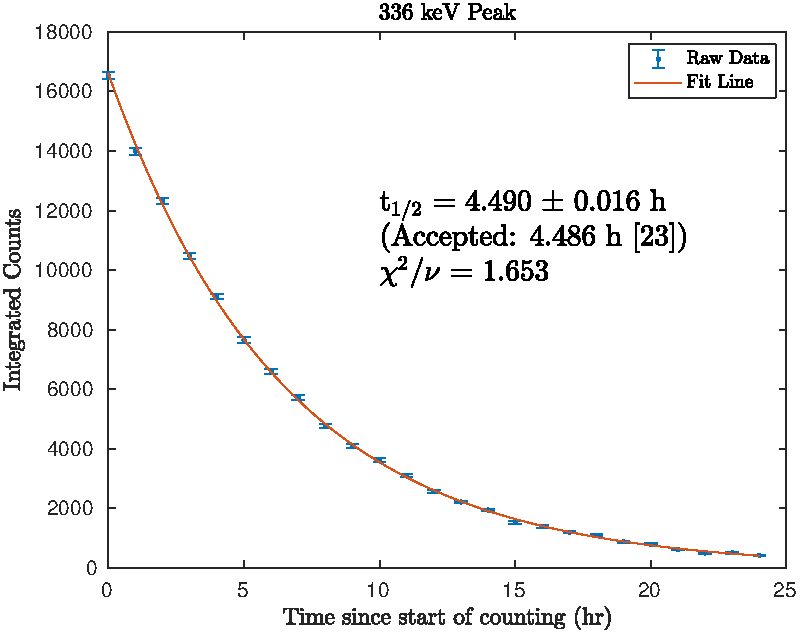
\includegraphics[scale=0.6]{./figures/336keV_curve_new.pdf}
        \caption{ Decay curve for the isomeric transition of \ce{^{115m}In}.}
        \label{fig:decay_curve_336}
    \end{subfigure}%
     \begin{subfigure}[t]{0.49\textwidth}
        \centering
%         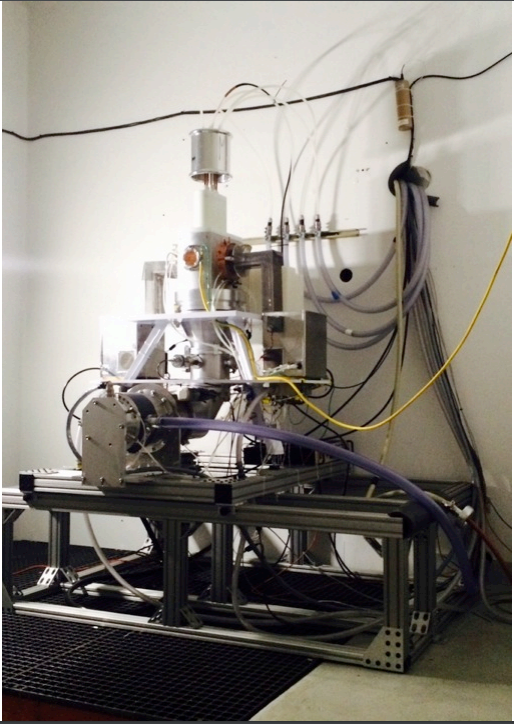
\includegraphics[width=\columnwidth]{./figures/Capture.PNG}
%         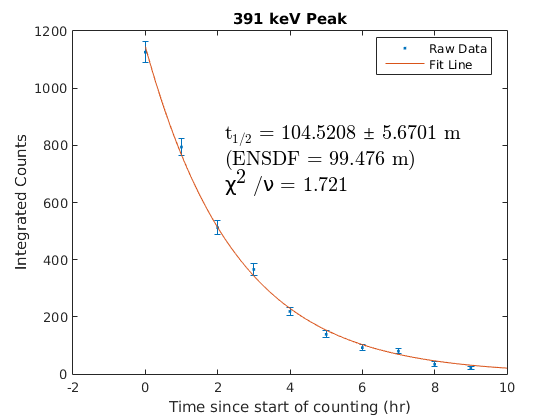
\includegraphics[scale=0.6]{./figures/391keV_curve2.png}
        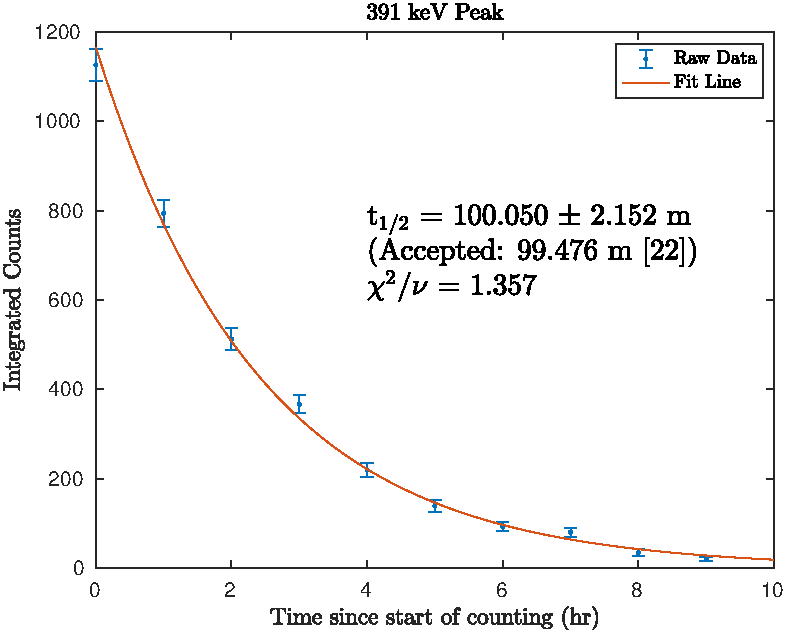
\includegraphics[scale=0.6]{./figures/391keV_curve_new.pdf}
        \caption{ Decay curve for the isomeric transition of \ce{^{113m}In}.}
        \label{fig:decay_curve_391}
    \end{subfigure}%
    \\
    \begin{subfigure}[t]{0.49\textwidth}
        \centering
%         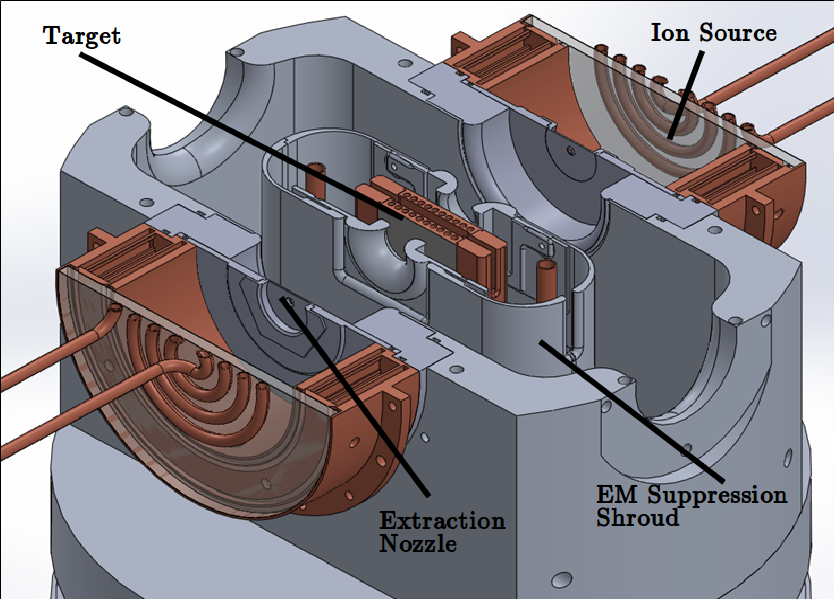
\includegraphics[width=\textwidth]{./figures/target2.png}
        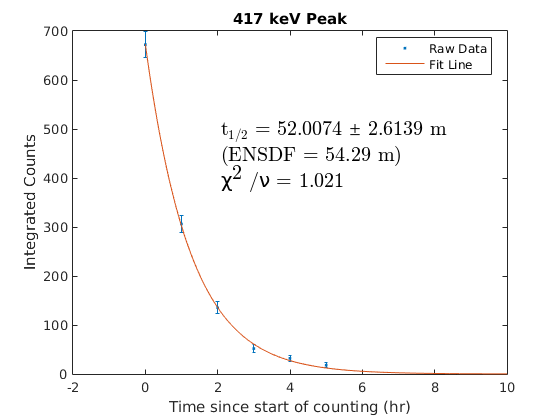
\includegraphics[scale=0.6]{./figures/417keV_curve2.png}
        \caption{Decay curve for the $\beta^-$ decay of \ce{^{116}In}.}
                \label{fig:decay_curve_417}
    \end{subfigure}
     \begin{subfigure}[t]{0.49\textwidth}
        \centering
%         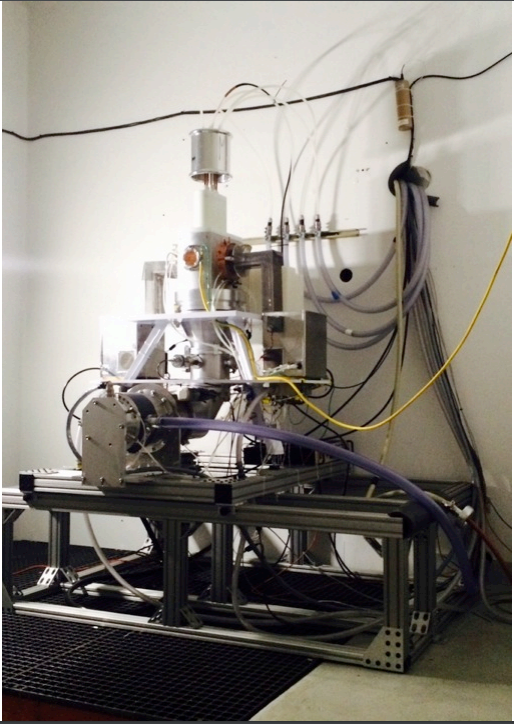
\includegraphics[width=\columnwidth]{./figures/Capture.PNG}
        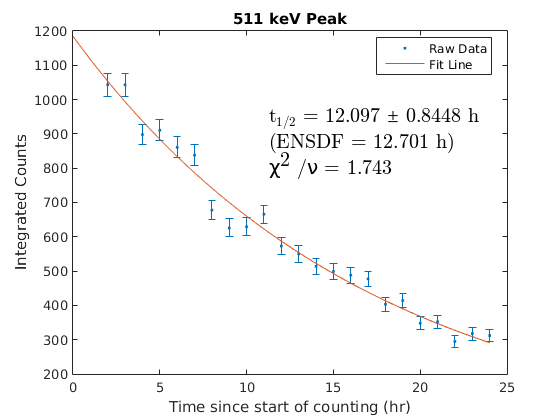
\includegraphics[scale=0.6]{./figures/511keV_curve2.png}
        \caption{ Decay curve for the $\beta^+$ decay of \ce{^{64}Cu}.}
        \label{fig:decay_curve_511}
    \end{subfigure}%
    \caption{Decay curves used to verify photopeak transition assignment.}
     \label{fig:decay_curves}
\end{figure*}

\comment{Need to update \autoref{fig:decay_curves} - figures are blurry}


The background-subtracted integrated counts in each photopeak, as well as the counting duration for each experiment, are tabulated in \autoref{tab:peak_counts}.

% Please add the following required packages to your document preamble:
% \usepackage{graphicx}
\begin{table*}
\centering
\caption{Counting times and photopeak counts for each of the (Zn/In) and (Ti/In)  experiments. \color{red}{Need Mauricio data!}}
\label{tab:peak_counts}
\resizebox{\textwidth}{!}{%
\begin{tabular}{c|ccccc}
Reference Foil                     & \ce{^{nat}In}         & \ce{^{nat}In}       & \ce{^{nat}In} & \ce{^{nat}In}     & \ce{^{nat}In}  \\ \hline
Reference Foil Mass (g)            & 0.248         & 0.248       & 0.241 & 0.247     & XXXXXX \\ \hline
Target Foil                        & \ce{^{nat}Zn}         & \ce{^{nat}Zn}       & \ce{^{nat}Zn} & \ce{^{nat}Ti}     & \ce{^{nat}Ti}  \\ \hline
Target Foil Mass (g)               & 0.538         & 0.451       & 0.452 & 0.337     & XXXX   \\ \hline
Irradiation Time, $t_1$ (s)           & 10800         & 10800       & 12629 & 11837     & XXXX   \\ \hline
Start of Count, $t_2$ (s)             & 12585         & 26985       & 14919 & 101245    & XXXX   \\ \hline
End of Count, $t_3$ (s)               & 103773        & 80993       & 68919 & 187669    & XXXX   \\ \hline
Photopeak Counts, 336 keV (\ce{^{115m}In}) & 113665 $\pm$ 1490 & 74321 $\pm$ 275 & XXXXX & 2122 $\pm$ 55 & XXXX   \\ \hline
Photopeak Counts, 391 keV (\ce{^{113m}In}) & 3382 $\pm$ 171    & 860 $\pm$ 40    & XXXXX &    \hrulefill       &  \hrulefill      \\ \hline
Photopeak Counts, 511 keV (\ce{^{64}Cu})   & 16055 $\pm$ 643   & 12852 $\pm$ 118 & XXXXX &    \hrulefill       &   \hrulefill     \\ \hline
Photopeak Counts, 159 keV (\ce{^{47}Sc})   &   \hrulefill            &    \hrulefill         &   \hrulefill    & 3877 $\pm$ 83 & XXXX  
\end{tabular}%
}
\end{table*}

% % Please add the following required packages to your document preamble:
% % \usepackage{booktabs}
% % \usepackage{graphicx}
% \begin{table*}
% \centering
% \caption{Counting times and photopeak counts for each of the (Zn/In) and (Ti/In)  experiments.}
% \label{tab:peak_counts}
% \resizebox{\textwidth}{!}{%
% \begin{tabular}{@{}|c|ccccc@{}}
% Reference Foil                     & natIn         & natIn       & natIn & natIn     & natIn  \\
% Reference Foil Mass (g)            & 0.248         & 0.248       & 0.241 & 0.247     & XXXXXX \\
% Target Foil                        & natZn         & natZn       & natZn & natTi     & natTi  \\
% Target Foil Mass (g)               & 0.538         & 0.451       & 0.452 & 0.337     & XXXX   \\
% Irradiation Time, t1 (s)           & 10800         & 10800       & 12629 & 11837     & XXXX   \\
% Start of Count, t2 (s)             & 12585         & 26985       & 14919 & 101245    & XXXX   \\
% End of Count, t3 (s)               & 103773        & 80993       & 68919 & 187669    & XXXX   \\
% Photopeak Counts, 336 keV (115mIn) & 113665 $\pm$ 1490 & 74321 $\pm$ 275 & XXXXX & 2122 $\pm$ 55 & XXXX   \\
% Photopeak Counts, 391 keV (113mIn) & 3382 $\pm$ 171    & 860 $\pm$ 40    & XXXXX &           &        \\
% Photopeak Counts, 511 keV (64Cu)   & 16055 $\pm$ 643   & 12852 $\pm$ 118 & XXXXX &           &        \\
% Photopeak Counts, 159 keV (47Sc)   &               &             &       & 3877 $\pm$ 83 & XXXX  
% \end{tabular}%
% }
% \end{table*}

\subsection{Calculation of measured cross sections}\label{sec:calcs_sec}


Gamma spectroscopy analysis on the several days of collected spectra was used to measure the background-subtracted counts under each of the photopeaks of interest for the induced activities, as described in \autoref{sec:spectroscopy}. For a thin target consisting of \(N_T\) target nuclei, subjected to a constant monoenergetic neutron flux $\phi\pp{\bar{E}}$, the rate of production of the product nucleus will be:

\begin{equation}
R = N_T \sigma\pp{\bar{E}} \phi\pp{\bar{E}} 
\end{equation}

for a reaction with cross-section  $\sigma\pp{\bar{E}}$ at effective energy $\bar{E}$. If this irradiation lasts for  some time $t_1$, and gamma ray spectroscopy of the activated samples begins at a later time $t_2$ and ends at an even later time $t_3$, then the number of product decays (with decay constant $\lambda$) which take place between $t_2$ and $t_3$ will be:



\begin{equation}
\begin{aligned}
D &= \dfrac{R}{\lambda}\pp{e^{\lambda t_1}-1}\pp{e^{-\lambda t_2} - e^{-\lambda t_3}}
\\
&= \dfrac{N_T \sigma\pp{\bar{E}} \phi\pp{\bar{E}} }{\lambda}\pp{e^{\lambda t_1}-1}\pp{e^{-\lambda t_2} - e^{-\lambda t_3}} 
\end{aligned}
\end{equation}

If this decay emits a gamma ray with branching ratio $I_\gamma$ photons emitted per decay, and is detected with an absolute efficiency (photons detected / photons emitted) of $\epsilon_\gamma$, then the number of observed decays between $t_2$ and $t_3$ will be:

% \begin{equation}
% \begin{aligned}
% N_{obs} &= D \epsilon_\gamma I_\gamma \\
% &= \? \epsilon_\gamma I_\gamma  \dfrac{N_T \sigma\pp{\bar{E}} \phi\pp{\bar{E}} }{\lambda}\pp{e^{\lambda t_1}-1}\pp{e^{-\lambda t_2} - e^{-\lambda t_3}} 
% \end{aligned}
% \end{equation}

\begin{align}
N_{obs} &= D \epsilon_\gamma I_\gamma \\
&=  \epsilon_\gamma I_\gamma  \dfrac{N_T \sigma\pp{\bar{E}} \phi\pp{\bar{E}} }{\lambda}\pp{e^{\lambda t_1}-1}\pp{e^{-\lambda t_2} - e^{-\lambda t_3}} \nonumber
\end{align}

Rearranging in terms of the observed cross-section:

\begin{equation}
\sigma\pp{\bar{E}} = \dfrac{N_{obs}\lambda}{N_T \epsilon_\gamma I_\gamma  \phi\pp{\bar{E}}  \pp{e^{\lambda t_1}-1}\pp{e^{-\lambda t_2} - e^{-\lambda t_3}}}
\end{equation}

This model, in which subscripts $P$ indicate a quantity for either the \ce{^{64}Cu} or \ce{^{47}Sc} product, subscripts $In$ indicate a quantity for either the \ce{^{113m}In} or \ce{^{115m}In} isomer, can be taken in ratio, to calculate the measured \ce{^{64}Zn}(n,p)\ce{^{64}Cu} and \ce{^{47}Ti}(n,p)\ce{^{47}Sc} production cross sections, relative to the \ce{^{113}In}(n,n')\ce{^{113m}In} and \ce{^{115}In}(n,n')\ce{^{115m}In} inelastic scattering cross sections. Adding in a correction for the small self-attenuation of the gamma rays emitted by the activated foils, the final ratio model can be seen in \autoref{eqn:calc_eqn}:

\begin{align}\label{eqn:calc_eqn}
\sigma_P &= \sigma_{In} \dfrac{A_P}{A_{In}} \dfrac{N_{T,In}}{N_{T,P}} \dfrac{\lambda_P}{\lambda_{In}} \dfrac{e^{\lambda_{In}t_1}-1}{e^{\lambda_{P}t_1}-1}  \\
&\times \dfrac{e^{-\lambda_{In}t_2}-e^{-\lambda_{In}t_3}}{e^{-\lambda_{P}t_2} - e^{-\lambda_{P}t_3}} \dfrac{\epsilon_{In}}{\epsilon_P}  \dfrac{I_{\gamma,In}}{I_{\gamma,P}} \dfrac{e^{-\mu_{In}x_{In}/2}\times e^{-\mu_{In}x_{P}}}{e^{-\mu_{P}x_{P}/2}} \nonumber
\end{align}

where:

\begin{itemize}
  

\item $A$ is the integrated counts under a photopeak [counts],

\item $\sigma$ is the cross section for either the production of a product or isomer [mb],

\item $N_T$ is the initial number of target nuclei,

\item $\lambda$  is the decay constant [s$^{-1}$],

\item $t_1$ is the irradiation time [s],

\item $t_2$ is the time between the start-of-beam and the start of counting [s],

\item $t_3$ is the time  between the start-of-beam and the end of counting [s],

\item $\epsilon$ is the  detector efficiency for a particular photopeak,

\item $I_\gamma$ is the decay gamma ray branching ratio,

\item $\mu$ is the photon attenuation coefficient for a particular decay gamma ray in a foil [cm$^{-1}$],

\item and $x$ is the thickness of foil traversed by a particular decay gamma ray [cm] 
\end{itemize}


With the exception of decay constants, which are assumed to be exact, each of the parameters in this model carries statistical uncertainty in measurement. In lieu of a differential error propagation, the total statistical error $\delta_\sigma$ is taken as the quadrature sum of all of the other errors  $\delta_i$:

\begin{equation}
\delta_\sigma = \norm{ \ensuremath{\vec{\delta}} }_2 = \sqrt{\sum_{i=1}^N  \delta_i^2  }
\end{equation}

This total statistical uncertainty will be plotted as the cross-section error bar in the excitation function for these production reactions.



\subsection{Systematic errors}

XXXXXXXXXXXXXXXX

\comment{Not sure what else we need to consider for systematics...}













\section{Results}


Using the ratio methods described here, the cross sections for the \ce{^{47}Ti}(n,p)\ce{^{47}Sc} and \ce{^{64}Zn}(n,p)\ce{^{64}Cu} reactions have been calculated for incident neutron energy of 2.7645 MeV,  + 0.0151 MeV / - 0.0219 MeV. These values are recorded in \autoref{tab:xs_results}.

\comment{Need Mauricio's Cu point w/ more sigfigs. Need Mauricio's Sc point too}

\comment{How many sig figs to round uncertainties to in table?}

\comment{Report all 3 values in table? Report a weighted average between them?}

% 
% % Please add the following required packages to your document preamble:
% % \usepackage{booktabs}
% \begin{table}[]
% \centering
% \caption{My caption}
% \label{my-label}
% \begin{tabular}{@{}cc@{}}
% \toprule
% h                                 & $\sigma$($E_n$ = 2.7645 MeV) (mb)                                                                     \\ \midrule
% \ce{^{64}Zn}(n,p)\ce{^{64}Cu} (relative to \ce{^{113}In}) & \begin{tabular}[c]{@{}c@{}}45.953 $\pm$ 3.351, \\ 46.493 $\pm$ 2.805, \\ 46.9 $\pm$ 3.189\end{tabular}  \\
% \ce{^{64}Zn}(n,p)\ce{^{64}Cu} (relative to \ce{^{115}In}) & \begin{tabular}[c]{@{}c@{}}49.716 $\pm$ 3.335, \\ 49.011 $\pm$ 2.698, \\ XXXX $\pm$ XXXXXX\end{tabular} \\
% \ce{^{47}Ti}(n,p)\ce{^{47}Sc} (relative to \ce{^{115}In}) & \begin{tabular}[c]{@{}c@{}}25.901 $\pm$ 1.7089, \\ XXXXX $\pm$ XXXXX\end{tabular}                   \\ \bottomrule
% \end{tabular}
% \end{table}


% Please add the following required packages to your document preamble:
% \usepackage{booktabs}
\begin{table}
\centering
\caption{Results of cross section measurement. }
\label{tab:xs_results}
\begin{tabular}{@{}cc@{}}
\toprule
Reaction                                                                            & $\sigma$($E_n$ = 2.7645 MeV) (mb)                                                                       \\ \midrule
\begin{tabular}[c]{@{}c@{}}\ce{^{64}Zn}(n,p)\ce{^{64}Cu} \\ (relative to \ce{^{113}In})\end{tabular} & \begin{tabular}[c]{@{}c@{}}45.953 $\pm$ 3.351, \\ 46.493 $\pm$ 2.805, \\ 46.9 $\pm$ 3.189\end{tabular}  \\
\begin{tabular}[c]{@{}c@{}}\ce{^{64}Zn}(n,p)\ce{^{64}Cu} \\ (relative to \ce{^{115}In})\end{tabular} & \begin{tabular}[c]{@{}c@{}}49.716 $\pm$ 3.335, \\ 49.011 $\pm$ 2.698, \\ XXXX $\pm$ XXXXXX\end{tabular} \\
\begin{tabular}[c]{@{}c@{}}\ce{^{47}Ti}(n,p)\ce{^{47}Sc} \\ (relative to \ce{^{115}In})\end{tabular} & \begin{tabular}[c]{@{}c@{}}25.901 $\pm$ 1.7089, \\ XXXXX $\pm$ XXXXX\end{tabular}                   \\ \bottomrule
\end{tabular}
\end{table}

The results for the \ce{^{47}Ti}(n,p)\ce{^{47}Sc} and \ce{^{64}Zn}(n,p)\ce{^{64}Cu} production cross sections can also be seen plotted in Figures \ref{fig:sc_xs} and \ref{fig:cu_xs}, respectively. It is apparent that the relative cross sections measured in the present work are consistent with both the small quantity of other literature results, and are measured to within 6\% uncertainty, lower than existing measurements. In addition, the results presented in this work show strong agreement with the recommended values from both the ENDF/B-VII.1 nuclear data library and reaction modeling results from TALYS\cite{koning2005talys}. 

\comment{Waiting on Lee for EMPIRE, ALICE data and language discussing differences and the significance of this.}


\comment{Mention Shimizu data specifically? }

\comment{Add a zoomed-in view like in \autoref{fig:cu_xs}?}

\begin{figure}
 \centering
 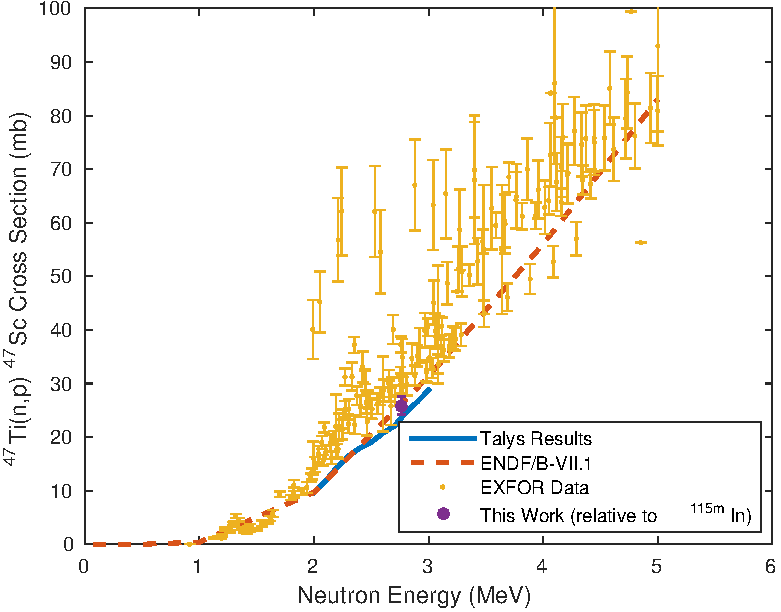
\includegraphics[scale=0.6]{./figures/47Sc_fixed.pdf}
 % 47Sc_fixed.pdf: 375x294 pixel, 72dpi, 13.23x10.37 cm, bb=0 0 375 294
 \caption{Measured \ce{^{47}Ti}(n,p)\ce{^{47}Sc} relative production cross section.}
 \label{fig:sc_xs}
\end{figure}

\begin{figure}
 \centering
 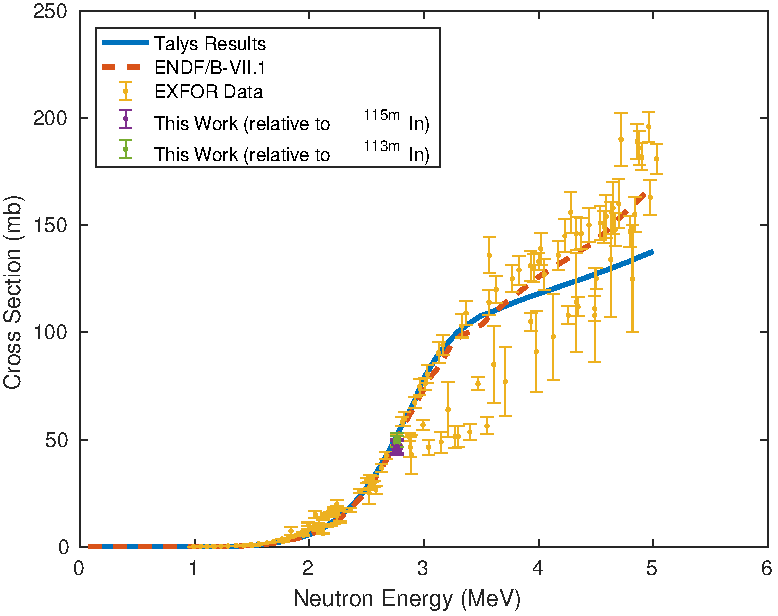
\includegraphics[scale=0.6]{./figures/64cu_fixed.pdf}
 % 47Sc_fixed.pdf: 375x294 pixel, 72dpi, 13.23x10.37 cm, bb=0 0 375 294
 \caption{Measured \ce{^{64}Zn}(n,p)\ce{^{64}Cu} relative production cross section}
 \label{fig:cu_xs}
\end{figure}


\begin{figure}
 \centering
 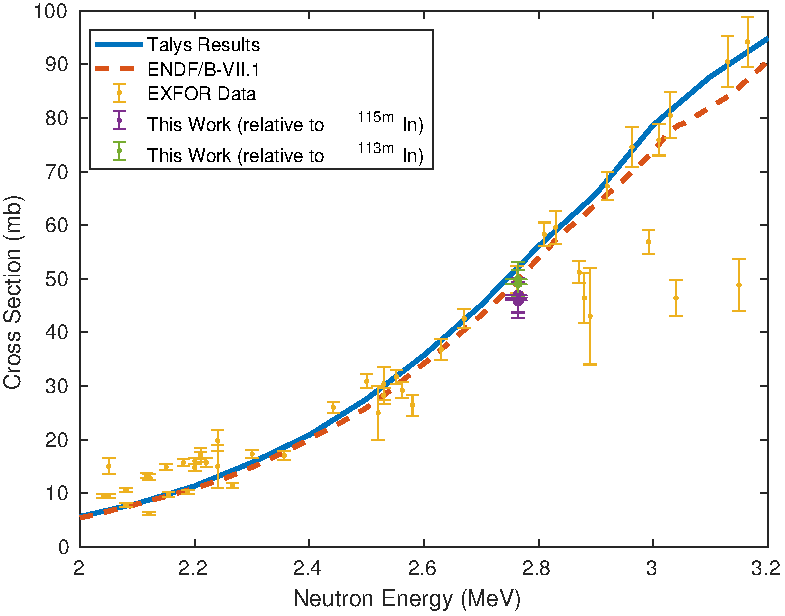
\includegraphics[scale=0.6]{./figures/64cu_fixed_zoom.pdf}
 % 47Sc_fixed.pdf: 375x294 pixel, 72dpi, 13.23x10.37 cm, bb=0 0 375 294
 \caption{A zoomed-in view of \autoref{fig:cu_xs}.}
 \label{fig:cu_xs_zoom}
\end{figure}





          
\section{Summary}

Using direct activation methods for thin foils as described in this work, the \ce{^{47}Ti}(n,p)\ce{^{47}Sc} and \ce{^{64}Zn}(n,p)\ce{^{64}Cu} production cross sections have been measured for  2.7645 MeV neutrons, to within 6\% uncertainty. These measurements are consistent with experimental data and theoretical models,  and have been measured to lower uncertainty than existing measurements. The use of DD neutron generators can be an efficient pathway for the measurement of these low-energy (n,p) reaction channels, as well as a relative method used to normalize measurements at higher neutron energies. While it reduces the neutron flux incident upon target foils, the use of collimated beam lines to irradiate foils at various angles allows a single neutron generator to perform these measurements at various other energies throughout the DD neutron emission energy spectrum. 

\comment{Future work? Thermal neutron measurements? Something like the following?}

 Future work will involve the continued measurement of the (n,p) production cross sections for various other emerging therapeutic and diagnostic radioisotopes, to expand the toolset of options available for modern medical imaging and cancer therapy. This will focus on radionuclides which permit more customized and precise dose deposition, as well as patient-specific treatments
 
 \comment{Should we specifically mention other isotopes we plan to measure?}


 
 \section{Acknowledgements}
 
 This work has been carried out at the University of California, Berkeley, and performed under the auspices of the U.S. Department of Energy by Lawrence Livermore National Laboratory under contract \# DE-AC52-07NA27344 and Lawrence Berkeley National Laboratory under contract \# DE-AC02-05CH11231. Funding has been provided from the US Nuclear Regulatory Commission and the US Nuclear Data Program.
 
 \comment{Who else should we acknowledge?}


% \pagebreak
% 
% \onecolumn
% 
% \appendix


% \section{Data} \label{data}
% 
% % \begin{longtable}{|c|c|c|c|c|} 
% % \caption{My caption}
% % \label{tab:dummy}
% % % \begin{tabular}{|c|c|c|c|c|}
% %    \hline
% %  
% % \end{longtable}
% hello world 

% 
% \section{Results} \label{equations}
% 
% Tabulated results are listed here, to avoid breaking text flow in the main text.
% 
% \begin{table}[h]
% \centering
% \caption{Transition conversion coefficients and efficiencies}
% \label{my-label2}
% \begin{tabular}{c|c|c|c|c}
% Nucleus & Transition       & E\(_\gamma\) (keV) & \(\alpha\), Conversion Coefficient  & \(\epsilon\), Intrinsic Efficiency \\ \hline
% \ce{^{110}Ru}   & 2\(\rightarrow\)0 & 240.7          & 0.0569           \(\pm\) 0.0008              & 1863.906   \\
%         & 4\(\rightarrow\)2 & 422.6          & 0.00887          \(\pm\) 0.00013             & 1219.507   \\
%         & 6\(\rightarrow\)4 & 575.7          & 0.00356          \(\pm\) 0.00005             & 956.569    \\ \hline
% \ce{^{140}Xe}   & 2\(\rightarrow\)0 & 376.657        & 0.0205          \(\pm\) 0.0003              & 1340.054   \\
%         & 4\(\rightarrow\)2 & 457.63         & 0.01154          \(\pm\) 0.00017             & 1142.505   \\
%         & 6\(\rightarrow\)4 & 582.4          & 0.00593          \(\pm\) 0.00009             & 948.705    \\ \hline
% \ce{^{140}Ba}   & 2\(\rightarrow\)0 & 602.35         & 0.00599         \(\pm\) 0.00009             & 926.624    \\
%         & 4\(\rightarrow\)2 & 528.25         & 0.00848         \(\pm\) 0.00012             & 1019.604   \\
%         & 6\(\rightarrow\)4 & 529.7          & 0.00842         \(\pm\) 0.00012             & 1017.470   \\ \hline
% \ce{^{144}Ba}   & 2\(\rightarrow\)0 & 199.326        & 0.175           \(\pm\) 0.0025              & 2085.452   \\
%         & 4\(\rightarrow\)2 & 330.88         & 0.0333         \(\pm\) 0.0005              & 1485.782   \\
%         & 6\(\rightarrow\)4 & 431.3          & 0.015          \(\pm\) 0.00021             & 1199.258  
% \end{tabular}
% \end{table}
% 
% \begin{table}[h]
% \centering
% \caption{Extracted transition intensities}
% \label{my-label}
% \begin{tabular}{c|c|c|c|c|c}
% Nucleus & Transition       & E\(_\gamma\) (keV) & \(A_{obs}\), Peak Area (a.u.)   & \(A_{source}\),  Peak Intensity (a.u.)  & \(R_i\), Relative Intensity  \\ \hline
% \ce{^{110}Ru}   & 2\(\rightarrow\)0 & 240.7          & 1097    \(\pm\)   136        & 0.622          \(\pm\) 0.077             & 1.000              \(\pm\) 0.175                 \\
%         & 4\(\rightarrow\)2 & 422.6          & 515     \(\pm\)   107        & 0.426          \(\pm\) 0.089             & 0.685              \(\pm\) 0.200                 \\
%         & 6\(\rightarrow\)4 & 575.7          & 144      \(\pm\)  55         & 0.151          \(\pm\) 0.058             & 0.243              \(\pm\) 0.198                 \\ \hline
% \ce{^{140}Xe}   & 2\(\rightarrow\)0 & 376.657        & 542     \(\pm\)   129        & 0.413          \(\pm\) 0.098             & 1.000              \(\pm\) 0.337                 \\
%         & 4\(\rightarrow\)2 & 457.63         & 357       \(\pm\) 59         & 0.316          \(\pm\) 0.052             & 0.766              \(\pm\) 0.254                 \\
%         & 6\(\rightarrow\)4 & 582.4          & 161       \(\pm\) 61         & 0.171          \(\pm\) 0.065             & 0.414              \(\pm\) 0.288                 \\ \hline
% \ce{^{140}Ba}   & 2\(\rightarrow\)0 & 602.35         & 822       \(\pm\) 164        & 0.892          \(\pm\) 0.178             & 1.000              \(\pm\) 0.282                 \\
%         & 4\(\rightarrow\)2 & 528.25         & 384       \(\pm\) 78         & 0.380          \(\pm\) 0.077             & 0.426              \(\pm\) 0.186                 \\
%         & 6\(\rightarrow\)4 & 529.7          & 310       \(\pm\) 104        & 0.307          \(\pm\) 0.103             & 0.344              \(\pm\) 0.229                 \\ \hline
% \ce{^{144}Ba}   & 2\(\rightarrow\)0 & 199.326        & 900       \(\pm\) 242        & 0.507          \(\pm\) 0.136             & 1.000              \(\pm\) 0.380                 \\
%         & 4\(\rightarrow\)2 & 330.88         & 535       \(\pm\) 127        & 0.372          \(\pm\) 0.088             & 0.734              \(\pm\) 0.307                 \\
%         & 6\(\rightarrow\)4 & 431.3          & 363       \(\pm\) 64         & 0.307          \(\pm\) 0.054             & 0.606              \(\pm\) 0.250                
% \end{tabular}
% \end{table}
%     
% \pagebreak
% 
% 
% 
% \section{Supplemental Figures} \label{fit_figures}
% 
% The remaining figures of the fitted \(\gamma\)-ray transition photopeaks are included here for reference, to avoid over-cluttering the main text.
% 
% 
% % \begin{figure}[h]
% %  \centering
% %  \includegraphics[scale=0.7]{./hw04/fit110Ru240-cropped.pdf}
% %  % fit110Ru240.ps: 570x750 pixel, 72dpi, 20.11x26.46 cm, bb=0 0 570 750
% %  \caption{Fit to the \ce{^{110}Ru} 240.7 keV peak and its surroundings.}
% %  \label{fig:110Ru240}
% % \end{figure}
% % 
% % \begin{figure}[h]
% %  \centering
% %  \includegraphics[scale=0.7]{./hw04/fit110Ru422-cropped.pdf}
% %  % fit110Ru240.ps: 570x750 pixel, 72dpi, 20.11x26.46 cm, bb=0 0 570 750
% %  \caption{Fit to the \ce{^{110}Ru} 422.6 keV peak and its surroundings.}
% %  \label{fig:110Ru422}
% % \end{figure}
% % 
% % \begin{figure}[h]
% %  \centering
% %  \includegraphics[scale=0.7]{./hw04/fit110Ru575-cropped.pdf}
% %  % fit110Ru240.ps: 570x750 pixel, 72dpi, 20.11x26.46 cm, bb=0 0 570 750
% %  \caption{Fit to the \ce{^{110}Ru} 575.7 keV peak and its surroundings.}
% %  \label{fig:110Ru575}
% % \end{figure}
% 
% 
% 
% 
% % \begin{figure}[h]
% %  \centering
% %  \includegraphics[scale=0.7]{./hw04/fit140Xe376-cropped.pdf}
% %  % fit110Ru240.ps: 570x750 pixel, 72dpi, 20.11x26.46 cm, bb=0 0 570 750
% %  \caption{Fit to the \ce{^{140}Xe} 376.7 keV peak and its surroundings.}
% %  \label{fig:140Xe376}
% % \end{figure}
% % 
% % \begin{figure}[h]
% %  \centering
% %  \includegraphics[scale=0.7]{./hw04/fit140Xe457-cropped.pdf}
% %  % fit110Ru240.ps: 570x750 pixel, 72dpi, 20.11x26.46 cm, bb=0 0 570 750
% %  \caption{Fit to the \ce{^{140}Xe} 457.6 keV peak and its surroundings.}
% %  \label{fig:140Xe457}
% % \end{figure}
% % 
% % \begin{figure}[h]
% %  \centering
% %  \includegraphics[scale=0.7]{./hw04/fit140Xe582-cropped.pdf}
% %  % fit110Ru240.ps: 570x750 pixel, 72dpi, 20.11x26.46 cm, bb=0 0 570 750
% %  \caption{Fit to the \ce{^{140}Xe} 582.3 keV peak and its surroundings.}
% %  \label{fig:140Xe582}
% % \end{figure}
% % 
% % 
% % 
% % \begin{figure}[h]
% %  \centering
% %  \includegraphics[scale=0.7]{./hw04/fit140Ba602-cropped.pdf}
% %  % fit110Ru240.ps: 570x750 pixel, 72dpi, 20.11x26.46 cm, bb=0 0 570 750
% %  \caption{Fit to the \ce{^{140}Ba} 602.4 keV peak and its surroundings.}
% %  \label{fig:140Ba602}
% % \end{figure}
% % 
% % 
% % 
% % 
% % 
% % \begin{figure}[h]
% %  \centering
% %  \includegraphics[scale=0.7]{./hw04/fit144Ba199-cropped.pdf}
% %  % fit110Ru240.ps: 570x750 pixel, 72dpi, 20.11x26.46 cm, bb=0 0 570 750
% %  \caption{Fit to the \ce{^{144}Ba} 199.3 keV peak and its surroundings.}
% %  \label{fig:144Ba199}
% % \end{figure}
% % 
% % 
% % 
% % \begin{figure}[h]
% %  \centering
% %  \includegraphics[scale=0.7]{./hw04/fit144Ba330-cropped.pdf}
% %  % fit110Ru240.ps: 570x750 pixel, 72dpi, 20.11x26.46 cm, bb=0 0 570 750
% %  \caption{Fit to the \ce{^{144}Ba} 330.9 keV peak and its surroundings.}
% %  \label{fig:144Ba330}
% % \end{figure}
% % 
% % \begin{figure}[h]
% %  \centering
% %  \includegraphics[scale=0.7]{./hw04/fit144Ba431-cropped.pdf}
% %  % fit110Ru240.ps: 570x750 pixel, 72dpi, 20.11x26.46 cm, bb=0 0 570 750
% %  \caption{Fit to the \ce{^{144}Ba} 431.3 keV peak and its surroundings.}
% %  \label{fig:144Ba431}
% % \end{figure}
% 
% 
% 
%     
% \pagebreak
% 
% 
% % \appendix
% \section{Source Code} \label{source}
% 
% \begin{center}
%  \texttt{gint.py} - Implementation of the Wilhelmy statistical model, used to estimate total transition intensities in the ground state band  of primary fission fragments
% \end{center}
% 
% % \begin{lstlisting}
% % \lstloadlanguages{Python}
% 
% % \lstinputlisting[linewidth=\columnwidth,language=Python,breaklines=true,frame=single]{./hw04/gint.py}
% % % \end{lstlisting}
% 
% 
% 
% \begin{center}
%  \texttt{hw04\_04.m} - used to process and plot statistical transition intensity curves
% \end{center}
% 
%  
% %   \lstinputlisting[frame=single]{./hw04/hw04_04.m}
% 
% 
% % \begin{verbatim}[commandchars=\\\{\}]
% % \verbatiminput{./HW01/test.txt}
% % \end{verbatim}
% 
% %% The Appendices part is started with the command \appendix;
% %% appendix sections are then done as normal sections
% %% \appendix
% 
% %% \section{}
% %% \label{}
% 
% %% References
% %%
% %% Following citation commands can be used in the body text:
% %% Usage of \cite is as follows:
% %%   \cite{key}         ==>>  [#]
% %%   \cite[chap. 2]{key} ==>> [#, chap. 2]
%%

% \twocolumn

%% References with BibTeX database:

% \bibliographystyle{elsarticle-num}
% \bibliographystyle{elsarticle-harv}
% \bibliographystyle{elsarticle-num-names}
% \bibliography{<your-bib-database>}
% \addcontentsline{toc}{chapter}{Bibliography}
% \bibliographystyle{elsarticle-num}
\bibliographystyle{ieeetr}
\bibliography{../../library}
% \thispagestyle{fancyTOC}



H. F. Aly et al., Microchim. Acta, vol. 59, no. 1, 1971.

K. S. Bhatki et al., J. Radioanal. Chem., vol. 2, no. 1-2, 1969.

T. H. Bokhari et al., J. Radioanal. Nucl. Chem., vol. 283, no. 2, 2010.

J. F. Briesmeister et al., Los Alamos National Laboratory, 1986.

M. B. Chadwick,et al., Nucl. Data Sheets, vol. 107, no. 12, 2006.

A. J. Koning et al., AIP Conference Proceedings, 2005, vol. 769, no. 2.

H. Liskien et al., Nucl. Data Tables, vol 11, 1973.

M. R. Lewis et al., J. Nucl. Med., vol. 44, no. 8, Aug. 2003.

C. Müller et al., J. Nucl. Med., vol. 55, no. 10, Oct. 2014.

N. Otuka et al., Nucl. Data Sheets, vol. 120, 2014.

L. Pietrelli et al., J. Radioanal. Nucl. Chem., vol. 157, no. 2, 1992.

S. M. Qaim et al., IAEA Technical Reports Series No. 473, 2011.

T. Shimizu, et al, Ann. Nucl. Energy, vol. 31, no. 9, pp. 975-990, 2004.

T. Shimizu, et al, Nucl. Instruments Methods Phys. Res. Sect. A Accel. Spectrometers, Detect. Assoc. Equip., vol. 527, no. 3, pp. 543-553, 2004.

D. Updegraff et al., ''Nuclear Medicine without Nuclear Reactors or Uranium Enrichment,'' 2013.


\comment{Cite Cory's thesis, or upcoming NIM paper?}

\comment{Convert these to BibTeX format!}

%% Authors are advised to use a BibTeX database file for their reference list.
%% The provided style file elsarticle-num.bst formats references in the required Procedia style

%% For references without a BibTeX database:

% \begin{thebibliography}{00}

%% \bibitem must have the following form:
%%   \bibitem{key}...
%% 

% \bibitem{}

% \end{thebibliography}

\end{document}

%%
%% End of file `ecrc-template.tex'. 